% Options for packages loaded elsewhere
\PassOptionsToPackage{unicode}{hyperref}
\PassOptionsToPackage{hyphens}{url}
%
\documentclass[
]{article}
\usepackage{lmodern}
\usepackage{amssymb,amsmath}
\usepackage{ifxetex,ifluatex}
\ifnum 0\ifxetex 1\fi\ifluatex 1\fi=0 % if pdftex
  \usepackage[T1]{fontenc}
  \usepackage[utf8]{inputenc}
  \usepackage{textcomp} % provide euro and other symbols
\else % if luatex or xetex
  \usepackage{unicode-math}
  \defaultfontfeatures{Scale=MatchLowercase}
  \defaultfontfeatures[\rmfamily]{Ligatures=TeX,Scale=1}
\fi
% Use upquote if available, for straight quotes in verbatim environments
\IfFileExists{upquote.sty}{\usepackage{upquote}}{}
\IfFileExists{microtype.sty}{% use microtype if available
  \usepackage[]{microtype}
  \UseMicrotypeSet[protrusion]{basicmath} % disable protrusion for tt fonts
}{}
\makeatletter
\@ifundefined{KOMAClassName}{% if non-KOMA class
  \IfFileExists{parskip.sty}{%
    \usepackage{parskip}
  }{% else
    \setlength{\parindent}{0pt}
    \setlength{\parskip}{6pt plus 2pt minus 1pt}}
}{% if KOMA class
  \KOMAoptions{parskip=half}}
\makeatother
\usepackage{xcolor}
\IfFileExists{xurl.sty}{\usepackage{xurl}}{} % add URL line breaks if available
\IfFileExists{bookmark.sty}{\usepackage{bookmark}}{\usepackage{hyperref}}
\hypersetup{
  hidelinks,
  pdfcreator={LaTeX via pandoc}}
\urlstyle{same} % disable monospaced font for URLs
\usepackage{longtable,booktabs}
% Correct order of tables after \paragraph or \subparagraph
\usepackage{etoolbox}
\makeatletter
\patchcmd\longtable{\par}{\if@noskipsec\mbox{}\fi\par}{}{}
\makeatother
% Allow footnotes in longtable head/foot
\IfFileExists{footnotehyper.sty}{\usepackage{footnotehyper}}{\usepackage{footnote}}
\makesavenoteenv{longtable}
\usepackage{graphicx,grffile}
\makeatletter
\def\maxwidth{\ifdim\Gin@nat@width>\linewidth\linewidth\else\Gin@nat@width\fi}
\def\maxheight{\ifdim\Gin@nat@height>\textheight\textheight\else\Gin@nat@height\fi}
\makeatother
% Scale images if necessary, so that they will not overflow the page
% margins by default, and it is still possible to overwrite the defaults
% using explicit options in \includegraphics[width, height, ...]{}
\setkeys{Gin}{width=\maxwidth,height=\maxheight,keepaspectratio}
% Set default figure placement to htbp
\makeatletter
\def\fps@figure{htbp}
\makeatother
\setlength{\emergencystretch}{3em} % prevent overfull lines
\providecommand{\tightlist}{%
  \setlength{\itemsep}{0pt}\setlength{\parskip}{0pt}}
\setcounter{secnumdepth}{-\maxdimen} % remove section numbering
%latex header to wrap code lines in .pdf

\usepackage{fvextra}
\DefineVerbatimEnvironment{Highlighting}{Verbatim}{breaklines,commandchars=\\\{\}}

\date{}

\begin{document}

\hypertarget{report-of-the-fit}{%
\section{Report of the fit}\label{report-of-the-fit}}

\hypertarget{fit-summary}{%
\subsection{Fit summary}\label{fit-summary}}

Description:\\
Minimiser: minuit\\
Random seed: 1234\\
Maximum values allowed for \(q_T / Q\): 0.2\\
Cut on the error function: 4\\
Parameterisation: PV19b\\
Explicit formula:

\[f_{\rm NP}(x,\zeta, b_T)= \Biggl((1-\lambda)
\left(\frac{1}{1 + g_1(x) b_T^2/4}+N_1\right) + \lambda \exp \left(-g_{1B}(x) b_T^2 /4 \right)\Biggr) \exp\left[- g_2 \log\left(\frac{\zeta}{Q_0^2}\right) b_T^2/4 - g_{2B} \log\left(\frac{\zeta}{Q_0^2}\right) b_T^4/4 \right]\]\[g_1(x) = \exp\left[\sigma\left(\frac{x}{\alpha}-1\right)\right]\]\[g_{1B}(x) = N_{1B} exp\left(-\frac{(x-\alpha_B)^2}{2\sigma_B^2}\right)\]\[Q_0^2 = 1\;{\rm GeV}^2\]
\(t_0\) prescription: True

\begin{longtable}[]{@{}ccccccccc@{}}
\toprule
\begin{minipage}[b]{0.09\columnwidth}\centering
\(g_2\)\strut
\end{minipage} & \begin{minipage}[b]{0.09\columnwidth}\centering
\(N_1\)\strut
\end{minipage} & \begin{minipage}[b]{0.09\columnwidth}\centering
\(\alpha\)\strut
\end{minipage} & \begin{minipage}[b]{0.08\columnwidth}\centering
\(\sigma\)\strut
\end{minipage} & \begin{minipage}[b]{0.08\columnwidth}\centering
\(\lambda\)\strut
\end{minipage} & \begin{minipage}[b]{0.07\columnwidth}\centering
\(N_{1B}\)\strut
\end{minipage} & \begin{minipage}[b]{0.08\columnwidth}\centering
\(\alpha_B\)\strut
\end{minipage} & \begin{minipage}[b]{0.09\columnwidth}\centering
\(\sigma_B\)\strut
\end{minipage} & \begin{minipage}[b]{0.09\columnwidth}\centering
\(g_{2B}\)\strut
\end{minipage}\tabularnewline
\midrule
\endhead
\begin{minipage}[t]{0.09\columnwidth}\centering
0.01637759456338\strut
\end{minipage} & \begin{minipage}[t]{0.09\columnwidth}\centering
-0.0360402603115\strut
\end{minipage} & \begin{minipage}[t]{0.09\columnwidth}\centering
0.07553836092907\strut
\end{minipage} & \begin{minipage}[t]{0.08\columnwidth}\centering
0.8738129447193\strut
\end{minipage} & \begin{minipage}[t]{0.08\columnwidth}\centering
0.7692672717837\strut
\end{minipage} & \begin{minipage}[t]{0.07\columnwidth}\centering
1.94666352759\strut
\end{minipage} & \begin{minipage}[t]{0.08\columnwidth}\centering
0.0900170221136\strut
\end{minipage} & \begin{minipage}[t]{0.09\columnwidth}\centering
0.03129685357799\strut
\end{minipage} & \begin{minipage}[t]{0.09\columnwidth}\centering
0.02024085243599\strut
\end{minipage}\tabularnewline
\bottomrule
\end{longtable}

\hypertarget{theory-summary}{%
\subsection{Theory summary}\label{theory-summary}}

Collinear PDF set: MMHT2014nnlo68cl member 0\\
Collinear FF set: DSS14\_NLO\_PiSum member 0\\
Perturbative order: N3LL\\
Reference value of the fine-structure constant:
\(\alpha(Q = 91.1876\;{\rm GeV}) = 0.00776578395589\) (running True)

\hypertarget{global-statistical-estimators}{%
\subsection{Global statistical
estimators}\label{global-statistical-estimators}}

\(N_{rep}\) = 247\\
\(\chi_{0}^2\) = 1.0063\\
\(\chi_{mean}^2\) = 0.9652\\
\(\langle\chi^2\rangle \pm \sigma_{\chi^2}\) = 1.0351 \(\pm\) 0.0147\\
\(\langle E \rangle \pm \sigma_{E}\) = 2.0165 \(\pm\) 0.1828

\hypertarget{parameters}{%
\subsection{Parameters}\label{parameters}}

\begin{longtable}[]{@{}cccc@{}}
\toprule
Parameter & Central replica & Average over replicas &
Fixed\tabularnewline
\midrule
\endhead
\(g_2\) & 0.016338215 & 0.01435339 \(\pm\) 0.01831858 &
False\tabularnewline
\(N_1\) & -0.035978765 & -0.03546671 \(\pm\) 0.00905085 &
False\tabularnewline
\(\alpha\) & 0.07543727 & 0.08182229 \(\pm\) 0.03354069 &
False\tabularnewline
\(\sigma\) & 0.87529147 & 1.04234075 \(\pm\) 1.39177636 &
False\tabularnewline
\(\lambda\) & 0.76896721 & 0.75375768 \(\pm\) 0.05763132 &
False\tabularnewline
\(N_{1B}\) & 1.9418189 & 2.54917603 \(\pm\) 2.16351415 &
False\tabularnewline
\(\alpha_B\) & 0.089887804 & 0.0904224 \(\pm\) 0.01219622 &
False\tabularnewline
\(\sigma_B\) & 0.031276945 & 0.02926968 \(\pm\) 0.00791431 &
False\tabularnewline
\(g_{2B}\) & 0.020236509 & 0.02029374 \(\pm\) 0.00427375 &
False\tabularnewline
\bottomrule
\end{longtable}

\begin{figure}
\centering
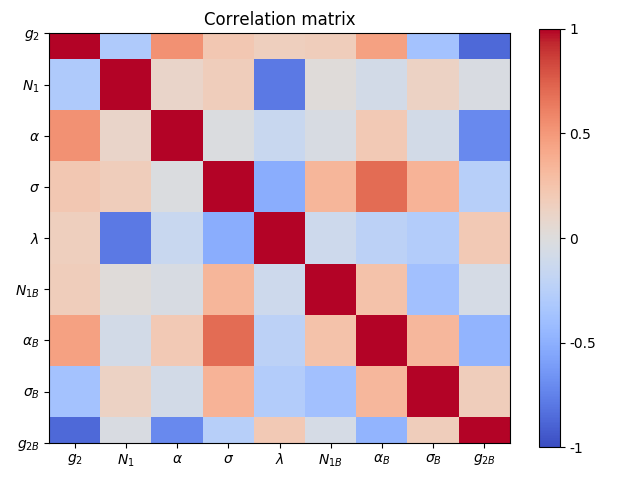
\includegraphics{pngplots/CorrelationMatrix.png}
\caption{Fitted parameter correlation matrix}
\end{figure}

\hypertarget{fit-properties}{%
\subsection{Fit properties}\label{fit-properties}}

\begin{figure}
\centering
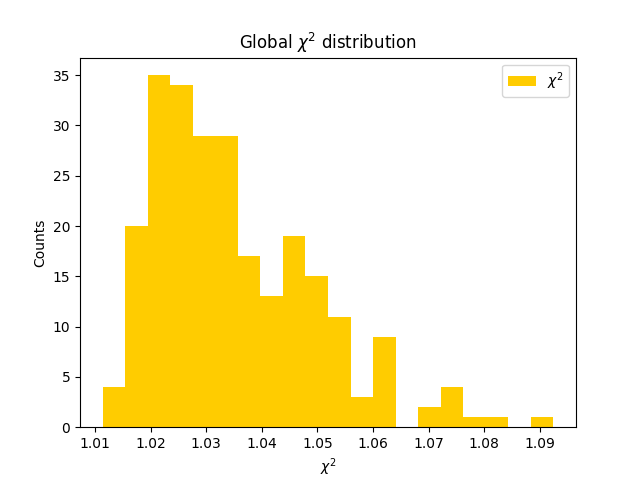
\includegraphics{pngplots/Globalchi2.png}
\caption{Global \(\chi^2\) distribution}
\end{figure}

\begin{figure}
\centering
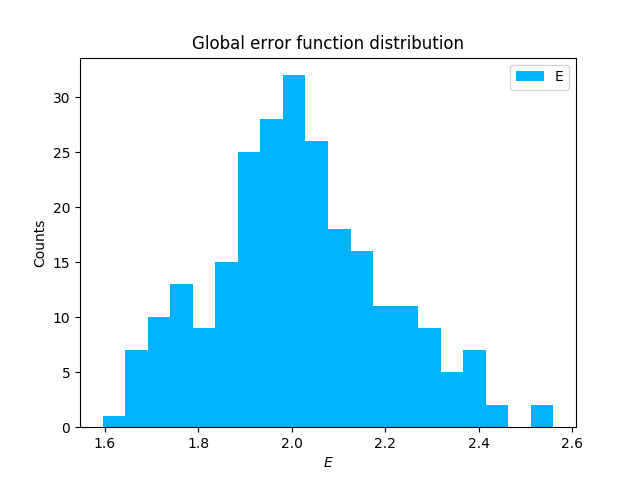
\includegraphics{pngplots/GlobalErrorFunction.png}
\caption{Global error function distribution}
\end{figure}

\begin{figure}
\centering
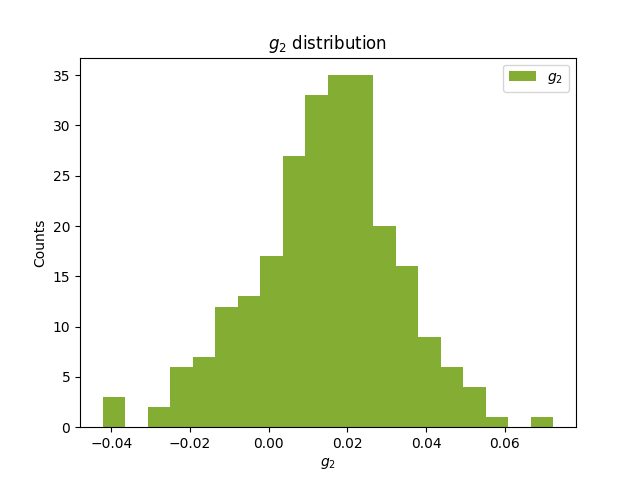
\includegraphics{pngplots/param0.png}
\caption{\(g_2\) distribution}
\end{figure}

\begin{figure}
\centering
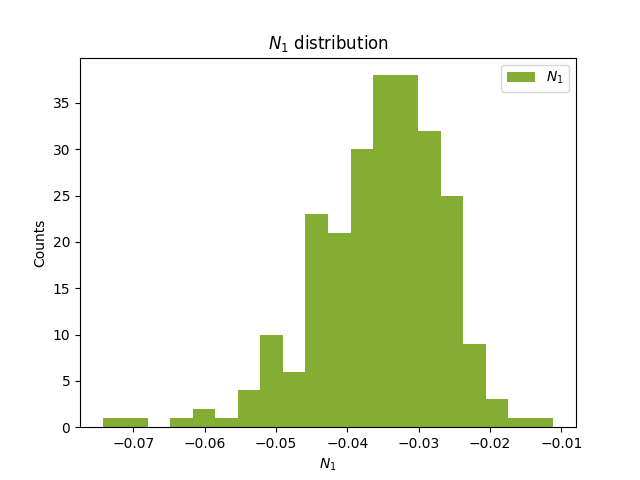
\includegraphics{pngplots/param1.png}
\caption{\(N_1\) distribution}
\end{figure}

\begin{figure}
\centering
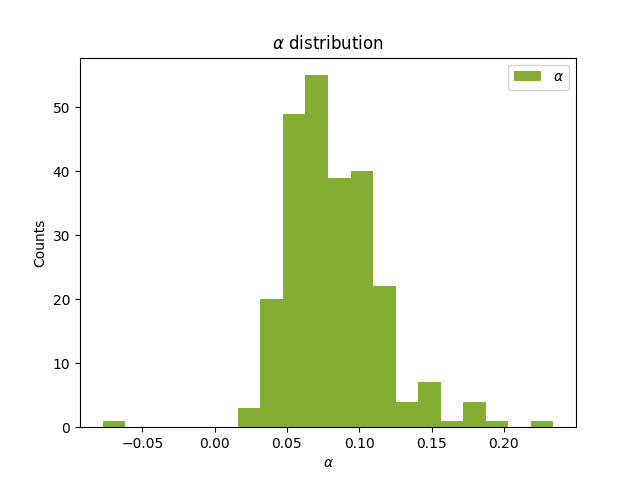
\includegraphics{pngplots/param2.png}
\caption{\(\alpha\) distribution}
\end{figure}

\begin{figure}
\centering
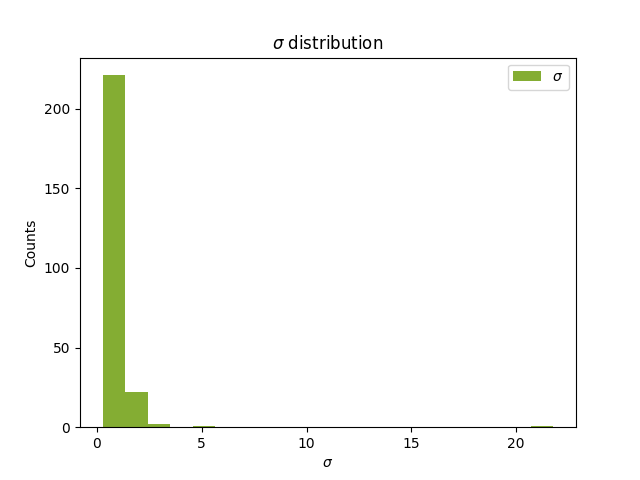
\includegraphics{pngplots/param3.png}
\caption{\(\sigma\) distribution}
\end{figure}

\begin{figure}
\centering
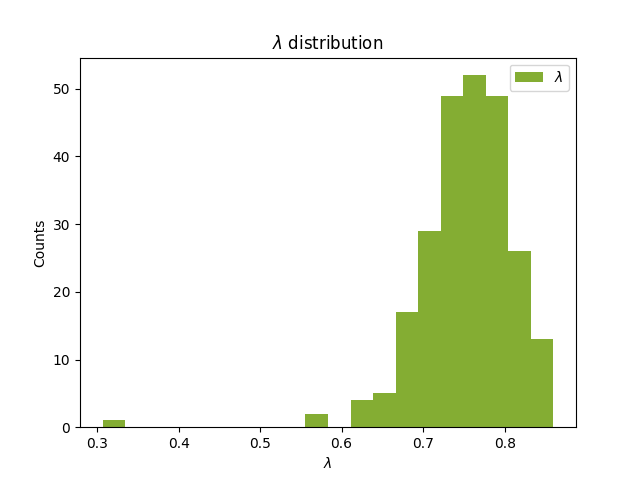
\includegraphics{pngplots/param4.png}
\caption{\(\lambda\) distribution}
\end{figure}

\begin{figure}
\centering
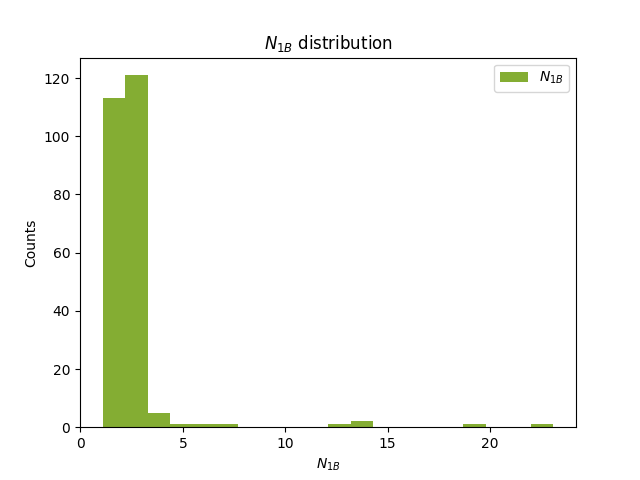
\includegraphics{pngplots/param5.png}
\caption{\(N_{1B}\) distribution}
\end{figure}

\begin{figure}
\centering
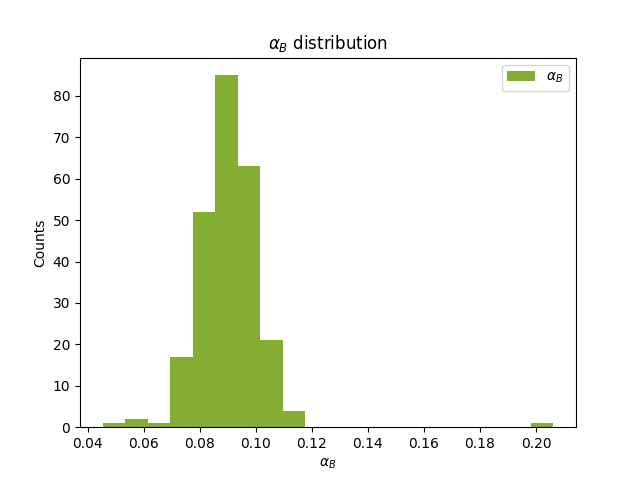
\includegraphics{pngplots/param6.png}
\caption{\(\alpha_B\) distribution}
\end{figure}

\begin{figure}
\centering
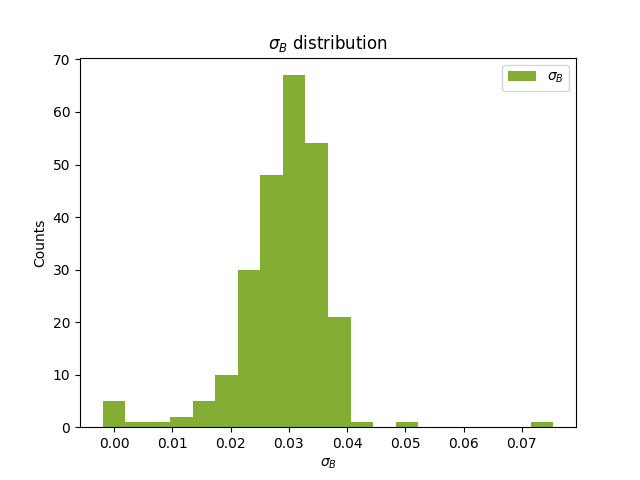
\includegraphics{pngplots/param7.png}
\caption{\(\sigma_B\) distribution}
\end{figure}

\begin{figure}
\centering
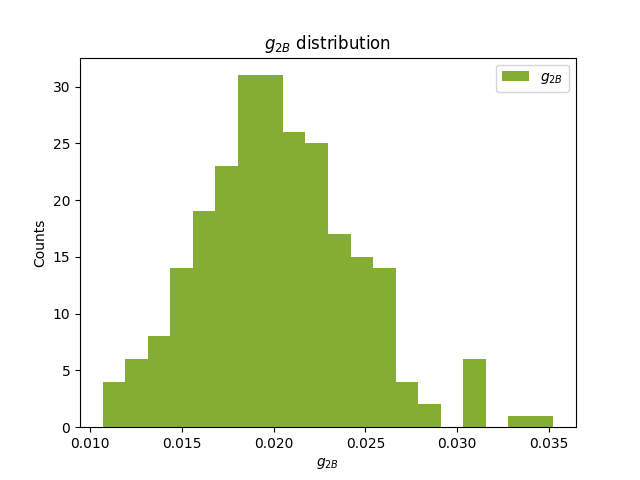
\includegraphics{pngplots/param8.png}
\caption{\(g_{2B}\) distribution}
\end{figure}

\hypertarget{table-of-chi2s}{%
\subsection{\texorpdfstring{Table of
\(\chi^2\)'s}{Table of \textbackslash chi\^{}2's}}\label{table-of-chi2s}}

Central-replica \(\chi^2\)'s:

\begin{longtable}[]{@{}ccccc@{}}
\toprule
Experiment & Number of points & \(\chi_{D}^2\) & \(\chi_{\lambda}^2\) &
\(\chi^2\)\tabularnewline
\midrule
\endhead
E605\_Q\_7\_8 & 7 & 0.4853 & 0.0883 & 0.5736\tabularnewline
E605\_Q\_8\_9 & 8 & 1.3747 & 0.1273 & 1.5021\tabularnewline
E605\_Q\_10.5\_11.5 & 10 & 0.7325 & 0.1384 & 0.8709\tabularnewline
E288\_200\_Q\_4\_5 & 4 & 1.0 & 0.8924 & 1.8924\tabularnewline
E288\_200\_Q\_5\_6 & 5 & 1.9025 & 0.2888 & 2.1914\tabularnewline
E288\_200\_Q\_6\_7 & 6 & 0.5848 & 0.3202 & 0.905\tabularnewline
E288\_200\_Q\_7\_8 & 7 & 0.7495 & 0.1079 & 0.8573\tabularnewline
E288\_200\_Q\_8\_9 & 8 & 0.6361 & 0.0041 & 0.6402\tabularnewline
E288\_300\_Q\_4\_5 & 4 & 0.8049 & 0.1324 & 0.9373\tabularnewline
E288\_300\_Q\_5\_6 & 5 & 1.0192 & 0.0001 & 1.0193\tabularnewline
E288\_300\_Q\_6\_7 & 6 & 0.6042 & 0.0016 & 0.6058\tabularnewline
E288\_300\_Q\_7\_8 & 7 & 0.1585 & 0.0383 & 0.1968\tabularnewline
E288\_300\_Q\_8\_9 & 8 & 0.458 & 0.0958 & 0.5538\tabularnewline
E288\_400\_Q\_5\_6 & 5 & 0.4662 & 0.1582 & 0.6245\tabularnewline
E288\_400\_Q\_6\_7 & 6 & 0.142 & 0.1153 & 0.2574\tabularnewline
E288\_400\_Q\_7\_8 & 7 & 0.0321 & 0.0772 & 0.1093\tabularnewline
E288\_400\_Q\_8\_9 & 8 & 0.5578 & 0.0334 & 0.5912\tabularnewline
E288\_400\_Q\_11\_12 & 11 & 0.4999 & 0.0193 & 0.5192\tabularnewline
E288\_400\_Q\_12\_13 & 12 & 0.5266 & 0.0284 & 0.555\tabularnewline
E288\_400\_Q\_13\_14 & 12 & 0.6506 & 0.0018 & 0.6524\tabularnewline
STAR\_510 & 7 & 1.2134 & 0.0468 & 1.2602\tabularnewline
CDF\_RunI & 25 & 0.5276 & 0.1116 & 0.6391\tabularnewline
CDF\_RunII & 26 & 0.7391 & 0.003 & 0.7421\tabularnewline
D0\_RunI & 12 & 0.5511 & 0.0092 & 0.5603\tabularnewline
D0\_RunII & 5 & 0.9851 & 0.2114 & 1.1965\tabularnewline
D0\_RunIImu & 3 & 4.0858 & 0.2928 & 4.3787\tabularnewline
LHCb\_7TeV & 7 & 1.1834 & 0.3566 & 1.54\tabularnewline
LHCb\_8TeV & 7 & 0.5522 & 0.4058 & 0.958\tabularnewline
LHCb\_13TeV & 7 & 0.929 & 0.0746 & 1.0036\tabularnewline
CMS\_7TeV & 4 & 2.8807 & 0 & 2.8807\tabularnewline
CMS\_8TeV & 4 & 1.1747 & 0.0019 & 1.1766\tabularnewline
ATLAS\_7TeV\_y\_0\_1 & 6 & 3.0305 & 0.4277 & 3.4582\tabularnewline
ATLAS\_7TeV\_y\_1\_2 & 6 & 1.9388 & 0.18 & 2.1188\tabularnewline
ATLAS\_7TeV\_y\_2\_2.4 & 6 & 1.8176 & 0.1651 & 1.9828\tabularnewline
ATLAS\_8TeV\_y\_0\_0.4 & 6 & 1.6387 & 0.0854 & 1.7241\tabularnewline
ATLAS\_8TeV\_y\_0.4\_0.8 & 6 & 1.6993 & 0.0659 & 1.7653\tabularnewline
ATLAS\_8TeV\_y\_0.8\_1.2 & 6 & 0.6021 & 0.0035 & 0.6056\tabularnewline
ATLAS\_8TeV\_y\_1.2\_1.6 & 6 & 0.7523 & 0.0326 & 0.7849\tabularnewline
ATLAS\_8TeV\_y\_1.6\_2 & 6 & 1.5223 & 0.0702 & 1.5926\tabularnewline
ATLAS\_8TeV\_y\_2\_2.4 & 6 & 0.7822 & 0.0694 & 0.8516\tabularnewline
ATLAS\_8TeV\_Q\_46\_66 & 4 & 1.206 & 0.328 & 1.5341\tabularnewline
ATLAS\_8TeV\_Q\_116\_150 & 8 & 0.7464 & 0.0563 & 0.8027\tabularnewline
Total & 319 & - & - & 1.0063\tabularnewline
\bottomrule
\end{longtable}

Mean-replica \(\chi^2\)'s:

\begin{longtable}[]{@{}ccccc@{}}
\toprule
Experiment & Number of points & \(\chi_{D}^2\) & \(\chi_{\lambda}^2\) &
\(\chi^2\)\tabularnewline
\midrule
\endhead
E605\_Q\_7\_8 & 7 & 0.5807 & 0.0473 & 0.628\tabularnewline
E605\_Q\_8\_9 & 8 & 1.6079 & 0.1303 & 1.7382\tabularnewline
E605\_Q\_10.5\_11.5 & 10 & 0.5775 & 0.081 & 0.6585\tabularnewline
E288\_200\_Q\_4\_5 & 4 & 0.4434 & 0.5186 & 0.962\tabularnewline
E288\_200\_Q\_5\_6 & 5 & 1.1685 & 0.1839 & 1.3525\tabularnewline
E288\_200\_Q\_6\_7 & 6 & 0.3329 & 0.1444 & 0.4773\tabularnewline
E288\_200\_Q\_7\_8 & 7 & 0.528 & 0.0569 & 0.5849\tabularnewline
E288\_200\_Q\_8\_9 & 8 & 0.6105 & 0.0039 & 0.6145\tabularnewline
E288\_300\_Q\_4\_5 & 4 & 0.5712 & 0.1672 & 0.7384\tabularnewline
E288\_300\_Q\_5\_6 & 5 & 1.0774 & 0.0009 & 1.0783\tabularnewline
E288\_300\_Q\_6\_7 & 6 & 0.596 & 0.0 & 0.5961\tabularnewline
E288\_300\_Q\_7\_8 & 7 & 0.1257 & 0.0142 & 0.1399\tabularnewline
E288\_300\_Q\_8\_9 & 8 & 0.3217 & 0.0484 & 0.3701\tabularnewline
E288\_400\_Q\_5\_6 & 5 & 0.8685 & 0.2345 & 1.103\tabularnewline
E288\_400\_Q\_6\_7 & 6 & 0.2158 & 0.2354 & 0.4512\tabularnewline
E288\_400\_Q\_7\_8 & 7 & 0.0545 & 0.1651 & 0.2195\tabularnewline
E288\_400\_Q\_8\_9 & 8 & 0.8189 & 0.071 & 0.8899\tabularnewline
E288\_400\_Q\_11\_12 & 11 & 0.4278 & 0.0081 & 0.4358\tabularnewline
E288\_400\_Q\_12\_13 & 12 & 0.4225 & 0.0185 & 0.441\tabularnewline
E288\_400\_Q\_13\_14 & 12 & 0.589 & 0.0118 & 0.6008\tabularnewline
STAR\_510 & 7 & 1.0218 & 0.091 & 1.1128\tabularnewline
CDF\_RunI & 25 & 0.4561 & 0.1157 & 0.5718\tabularnewline
CDF\_RunII & 26 & 0.712 & 0.0026 & 0.7146\tabularnewline
D0\_RunI & 12 & 0.5555 & 0.0048 & 0.5603\tabularnewline
D0\_RunII & 5 & 1.1137 & 0.1824 & 1.2961\tabularnewline
D0\_RunIImu & 3 & 4.1618 & 0.3745 & 4.5363\tabularnewline
LHCb\_7TeV & 7 & 1.0844 & 0.4141 & 1.4984\tabularnewline
LHCb\_8TeV & 7 & 0.4985 & 0.4511 & 0.9496\tabularnewline
LHCb\_13TeV & 7 & 0.8621 & 0.084 & 0.9461\tabularnewline
CMS\_7TeV & 4 & 3.05 & 0 & 3.05\tabularnewline
CMS\_8TeV & 4 & 1.1929 & 0.0053 & 1.1982\tabularnewline
ATLAS\_7TeV\_y\_0\_1 & 6 & 3.4663 & 0.6005 & 4.0668\tabularnewline
ATLAS\_7TeV\_y\_1\_2 & 6 & 1.7382 & 0.1102 & 1.8485\tabularnewline
ATLAS\_7TeV\_y\_2\_2.4 & 6 & 1.6373 & 0.1396 & 1.7769\tabularnewline
ATLAS\_8TeV\_y\_0\_0.4 & 6 & 1.8327 & 0.165 & 1.9977\tabularnewline
ATLAS\_8TeV\_y\_0.4\_0.8 & 6 & 1.7847 & 0.1639 & 1.9486\tabularnewline
ATLAS\_8TeV\_y\_0.8\_1.2 & 6 & 0.624 & 0.0009 & 0.625\tabularnewline
ATLAS\_8TeV\_y\_1.2\_1.6 & 6 & 0.6922 & 0.0106 & 0.7028\tabularnewline
ATLAS\_8TeV\_y\_1.6\_2 & 6 & 1.171 & 0.0408 & 1.2118\tabularnewline
ATLAS\_8TeV\_y\_2\_2.4 & 6 & 0.6674 & 0.0855 & 0.7529\tabularnewline
ATLAS\_8TeV\_Q\_46\_66 & 4 & 1.1693 & 0.2492 & 1.4185\tabularnewline
ATLAS\_8TeV\_Q\_116\_150 & 8 & 0.7933 & 0.084 & 0.8773\tabularnewline
Total & 319 & - & - & 0.9652\tabularnewline
\bottomrule
\end{longtable}

Average-over-replicas \(\chi^2\)'s:

\begin{longtable}[]{@{}ccccc@{}}
\toprule
Experiment & Number of points & \(\chi_{D}^2\) & \(\chi_{\lambda}^2\) &
\(\chi^2\)\tabularnewline
\midrule
\endhead
E605\_Q\_7\_8 & 7 & 0.4567 \(\pm\) 0.2986 & 0.2365 \(\pm\) 0.2848 &
0.6932 \(\pm\) 0.191\tabularnewline
E605\_Q\_8\_9 & 8 & 1.3088 \(\pm\) 0.3393 & 0.1978 \(\pm\) 0.2141 &
1.5066 \(\pm\) 0.3109\tabularnewline
E605\_Q\_10.5\_11.5 & 10 & 0.6653 \(\pm\) 0.3202 & 0.2215 \(\pm\) 0.2782
& 0.8868 \(\pm\) 0.1513\tabularnewline
E288\_200\_Q\_4\_5 & 4 & 0.5634 \(\pm\) 1.6577 & 1.3585 \(\pm\) 1.4892 &
1.9219 \(\pm\) 0.6035\tabularnewline
E288\_200\_Q\_5\_6 & 5 & 1.6557 \(\pm\) 0.8453 & 0.591 \(\pm\) 0.7852 &
2.2466 \(\pm\) 0.2487\tabularnewline
E288\_200\_Q\_6\_7 & 6 & 0.3644 \(\pm\) 0.6526 & 0.5633 \(\pm\) 0.6338 &
0.9277 \(\pm\) 0.1542\tabularnewline
E288\_200\_Q\_7\_8 & 7 & 0.5948 \(\pm\) 0.3856 & 0.2763 \(\pm\) 0.3564 &
0.8711 \(\pm\) 0.1252\tabularnewline
E288\_200\_Q\_8\_9 & 8 & 0.5402 \(\pm\) 0.1389 & 0.1108 \(\pm\) 0.1352 &
0.651 \(\pm\) 0.0425\tabularnewline
E288\_300\_Q\_4\_5 & 4 & 0.5962 \(\pm\) 0.6501 & 0.3672 \(\pm\) 0.5359 &
0.9635 \(\pm\) 0.3342\tabularnewline
E288\_300\_Q\_5\_6 & 5 & 0.8638 \(\pm\) 0.3242 & 0.1896 \(\pm\) 0.2575 &
1.0534 \(\pm\) 0.1828\tabularnewline
E288\_300\_Q\_6\_7 & 6 & 0.4667 \(\pm\) 0.2807 & 0.1503 \(\pm\) 0.2178 &
0.617 \(\pm\) 0.1646\tabularnewline
E288\_300\_Q\_7\_8 & 7 & 0.0187 \(\pm\) 0.2534 & 0.1927 \(\pm\) 0.2374 &
0.2114 \(\pm\) 0.0694\tabularnewline
E288\_300\_Q\_8\_9 & 8 & 0.3542 \(\pm\) 0.3112 & 0.2188 \(\pm\) 0.3076 &
0.573 \(\pm\) 0.0739\tabularnewline
E288\_400\_Q\_5\_6 & 5 & 0.4049 \(\pm\) 0.3488 & 0.2576 \(\pm\) 0.3075 &
0.6626 \(\pm\) 0.1593\tabularnewline
E288\_400\_Q\_6\_7 & 6 & 0.0975 \(\pm\) 0.2244 & 0.1979 \(\pm\) 0.2129 &
0.2954 \(\pm\) 0.0882\tabularnewline
E288\_400\_Q\_7\_8 & 7 & -0.0376 \(\pm\) 0.2371 & 0.1887 \(\pm\) 0.2302
& 0.151 \(\pm\) 0.0683\tabularnewline
E288\_400\_Q\_8\_9 & 8 & 0.4816 \(\pm\) 0.1969 & 0.1329 \(\pm\) 0.1798 &
0.6145 \(\pm\) 0.0946\tabularnewline
E288\_400\_Q\_11\_12 & 11 & 0.4138 \(\pm\) 0.188 & 0.1149 \(\pm\) 0.1637
& 0.5287 \(\pm\) 0.0864\tabularnewline
E288\_400\_Q\_12\_13 & 12 & 0.4724 \(\pm\) 0.1625 & 0.1151 \(\pm\)
0.1455 & 0.5874 \(\pm\) 0.0696\tabularnewline
E288\_400\_Q\_13\_14 & 12 & 0.6154 \(\pm\) 0.1094 & 0.0608 \(\pm\)
0.0793 & 0.6762 \(\pm\) 0.0655\tabularnewline
STAR\_510 & 7 & 1.1208 \(\pm\) 0.2381 & 0.1503 \(\pm\) 0.2193 & 1.2711
\(\pm\) 0.0961\tabularnewline
CDF\_RunI & 25 & 0.4862 \(\pm\) 0.1362 & 0.1572 \(\pm\) 0.1338 & 0.6434
\(\pm\) 0.0197\tabularnewline
CDF\_RunII & 26 & 0.7116 \(\pm\) 0.0827 & 0.0525 \(\pm\) 0.0668 & 0.7641
\(\pm\) 0.0519\tabularnewline
D0\_RunI & 12 & 0.5046 \(\pm\) 0.0953 & 0.0665 \(\pm\) 0.0887 & 0.5711
\(\pm\) 0.0304\tabularnewline
D0\_RunII & 5 & 0.7724 \(\pm\) 0.5424 & 0.4217 \(\pm\) 0.5215 & 1.194
\(\pm\) 0.1951\tabularnewline
D0\_RunIImu & 3 & 3.5218 \(\pm\) 0.9145 & 0.8055 \(\pm\) 0.6553 & 4.3272
\(\pm\) 0.5973\tabularnewline
LHCb\_7TeV & 7 & 0.9881 \(\pm\) 0.4896 & 0.5837 \(\pm\) 0.4834 & 1.5718
\(\pm\) 0.0568\tabularnewline
LHCb\_8TeV & 7 & 0.4674 \(\pm\) 0.5374 & 0.5273 \(\pm\) 0.508 & 0.9947
\(\pm\) 0.1554\tabularnewline
LHCb\_13TeV & 7 & 0.8601 \(\pm\) 0.2596 & 0.166 \(\pm\) 0.2556 & 1.0261
\(\pm\) 0.099\tabularnewline
CMS\_7TeV & 4 & 2.8893 \(\pm\) 0.1278 & 0.0 \(\pm\) 0.0 & 2.8893 \(\pm\)
0.1278\tabularnewline
CMS\_8TeV & 4 & 1.1036 \(\pm\) 0.1147 & 0.0697 \(\pm\) 0.0978 & 1.1734
\(\pm\) 0.0614\tabularnewline
ATLAS\_7TeV\_y\_0\_1 & 6 & 3.0166 \(\pm\) 0.5612 & 0.4954 \(\pm\) 0.3277
& 3.512 \(\pm\) 0.4314\tabularnewline
ATLAS\_7TeV\_y\_1\_2 & 6 & 1.9898 \(\pm\) 0.3105 & 0.2132 \(\pm\) 0.1873
& 2.2031 \(\pm\) 0.2402\tabularnewline
ATLAS\_7TeV\_y\_2\_2.4 & 6 & 1.8735 \(\pm\) 0.2182 & 0.1937 \(\pm\)
0.1078 & 2.0673 \(\pm\) 0.1949\tabularnewline
ATLAS\_8TeV\_y\_0\_0.4 & 6 & 1.6357 \(\pm\) 0.3136 & 0.1326 \(\pm\)
0.1498 & 1.7683 \(\pm\) 0.2708\tabularnewline
ATLAS\_8TeV\_y\_0.4\_0.8 & 6 & 1.7013 \(\pm\) 0.2211 & 0.1413 \(\pm\)
0.1752 & 1.8426 \(\pm\) 0.1577\tabularnewline
ATLAS\_8TeV\_y\_0.8\_1.2 & 6 & 0.6011 \(\pm\) 0.0917 & 0.0418 \(\pm\)
0.0634 & 0.6429 \(\pm\) 0.0671\tabularnewline
ATLAS\_8TeV\_y\_1.2\_1.6 & 6 & 0.7428 \(\pm\) 0.1546 & 0.0831 \(\pm\)
0.101 & 0.8259 \(\pm\) 0.1238\tabularnewline
ATLAS\_8TeV\_y\_1.6\_2 & 6 & 1.5167 \(\pm\) 0.4534 & 0.1713 \(\pm\)
0.1887 & 1.688 \(\pm\) 0.3995\tabularnewline
ATLAS\_8TeV\_y\_2\_2.4 & 6 & 0.8097 \(\pm\) 0.4102 & 0.1313 \(\pm\)
0.1506 & 0.941 \(\pm\) 0.385\tabularnewline
ATLAS\_8TeV\_Q\_46\_66 & 4 & 1.0623 \(\pm\) 0.5298 & 0.4723 \(\pm\)
0.4924 & 1.5346 \(\pm\) 0.1621\tabularnewline
ATLAS\_8TeV\_Q\_116\_150 & 8 & 0.6653 \(\pm\) 0.2296 & 0.1558 \(\pm\)
0.2095 & 0.8211 \(\pm\) 0.0851\tabularnewline
Total & 319 & - & - & 1.0351 \(\pm\) 0.0147\tabularnewline
\bottomrule
\end{longtable}

\hypertarget{tmds-in-k_t-space}{%
\subsection{\texorpdfstring{TMDs in \(k_T\)
space}{TMDs in k\_T space}}\label{tmds-in-k_t-space}}

\begin{figure}
\centering
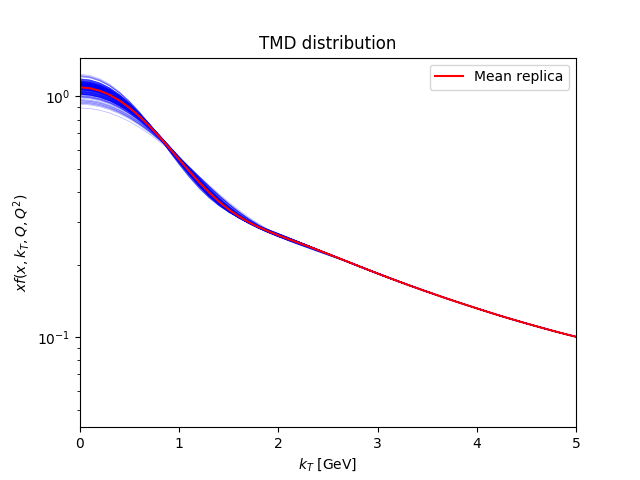
\includegraphics{pngplots/tmd_1_2_0.001.png}
\caption{TMD PDF of the \(d\) at \(Q = 2\) GeV and \(x = 0.001\)}
\end{figure}

\begin{figure}
\centering
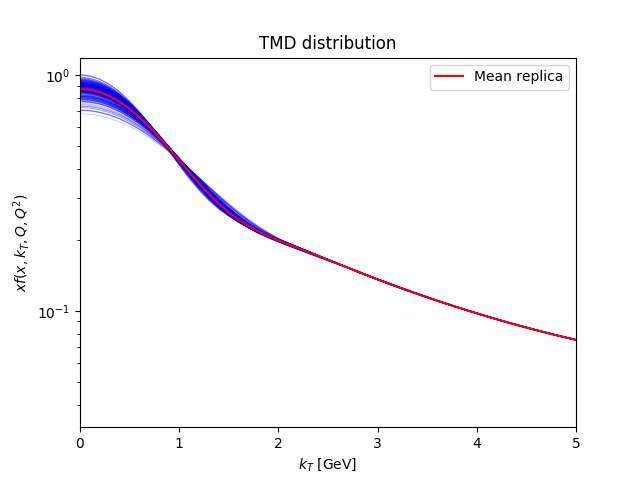
\includegraphics{pngplots/tmd_1_2_0.01.png}
\caption{TMD PDF of the \(d\) at \(Q = 2\) GeV and \(x = 0.01\)}
\end{figure}

\begin{figure}
\centering
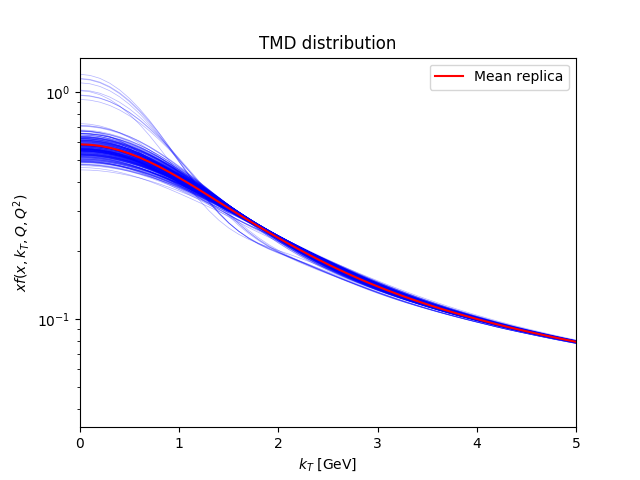
\includegraphics{pngplots/tmd_1_2_0.1.png}
\caption{TMD PDF of the \(d\) at \(Q = 2\) GeV and \(x = 0.1\)}
\end{figure}

\begin{figure}
\centering
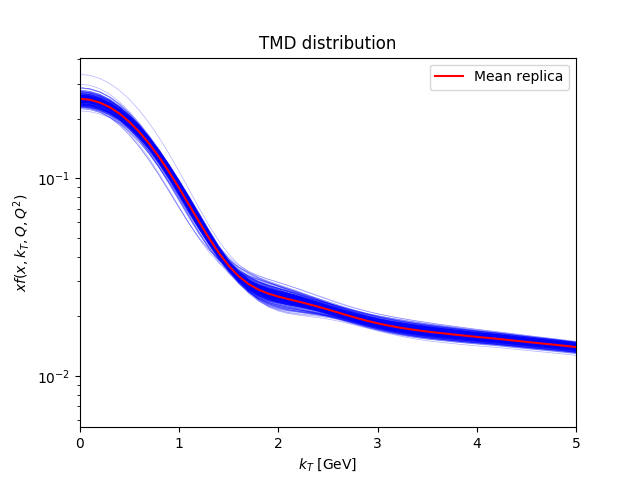
\includegraphics{pngplots/tmd_1_2_0.5.png}
\caption{TMD PDF of the \(d\) at \(Q = 2\) GeV and \(x = 0.5\)}
\end{figure}

\begin{figure}
\centering
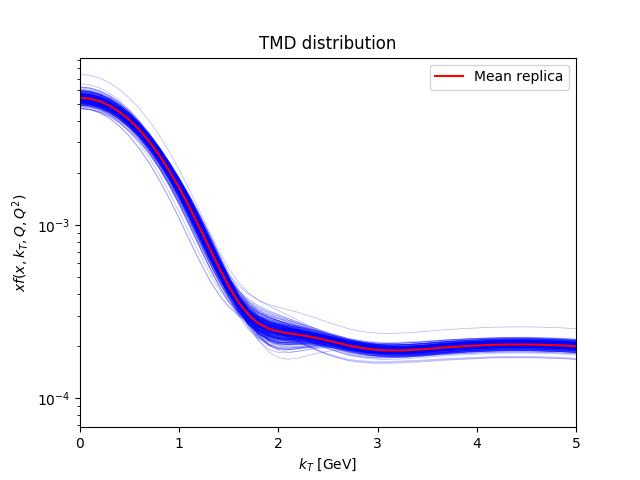
\includegraphics{pngplots/tmd_1_2_0.9.png}
\caption{TMD PDF of the \(d\) at \(Q = 2\) GeV and \(x = 0.9\)}
\end{figure}

\hypertarget{data-theory-comparison}{%
\subsection{Data-theory comparison}\label{data-theory-comparison}}

\begin{figure}
\centering
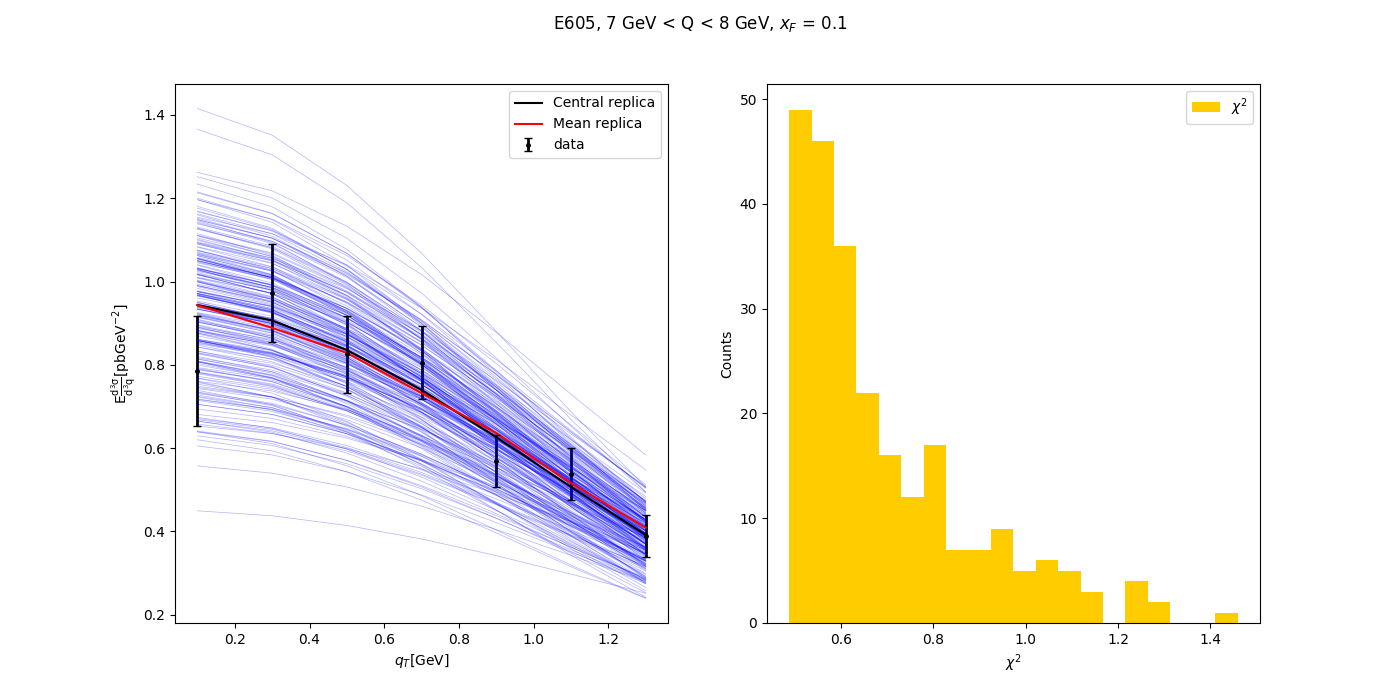
\includegraphics{pngplots/E605_Q_7_8.png}
\caption{E605\_Q\_7\_8 data-theory comparison}
\end{figure}

\begin{figure}
\centering
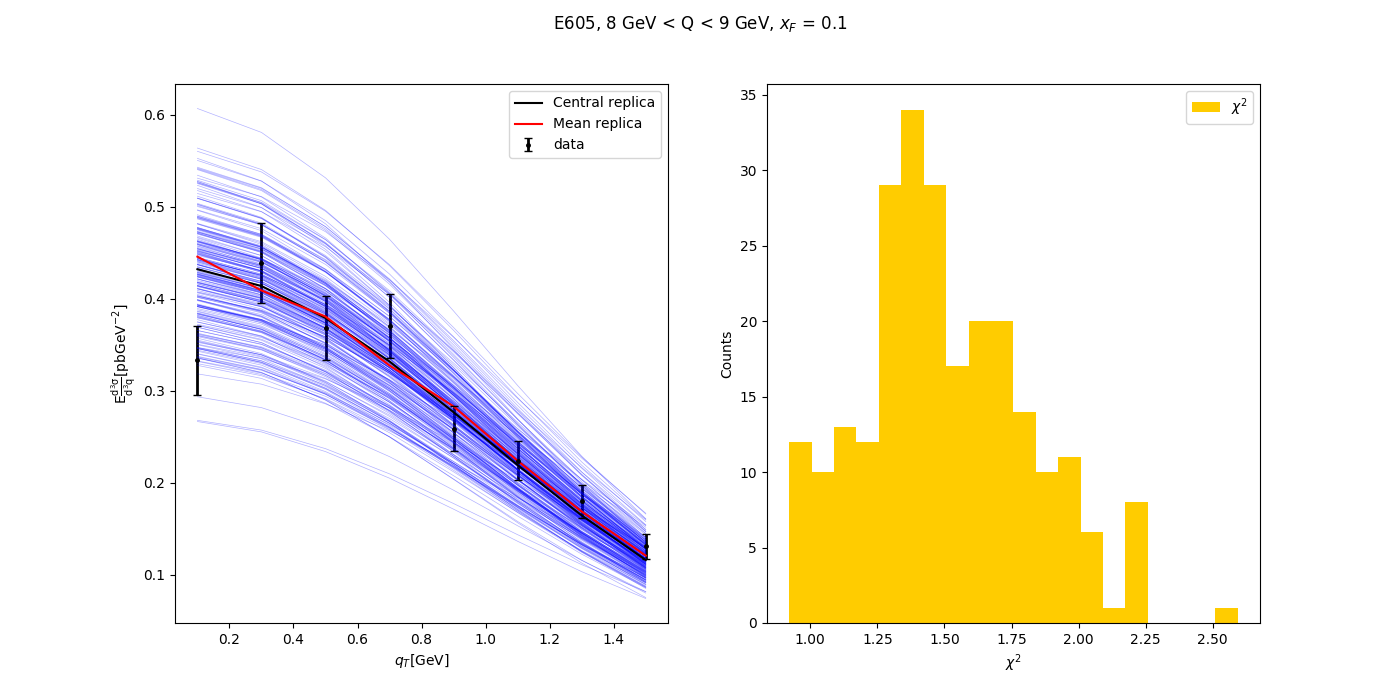
\includegraphics{pngplots/E605_Q_8_9.png}
\caption{E605\_Q\_8\_9 data-theory comparison}
\end{figure}

\begin{figure}
\centering
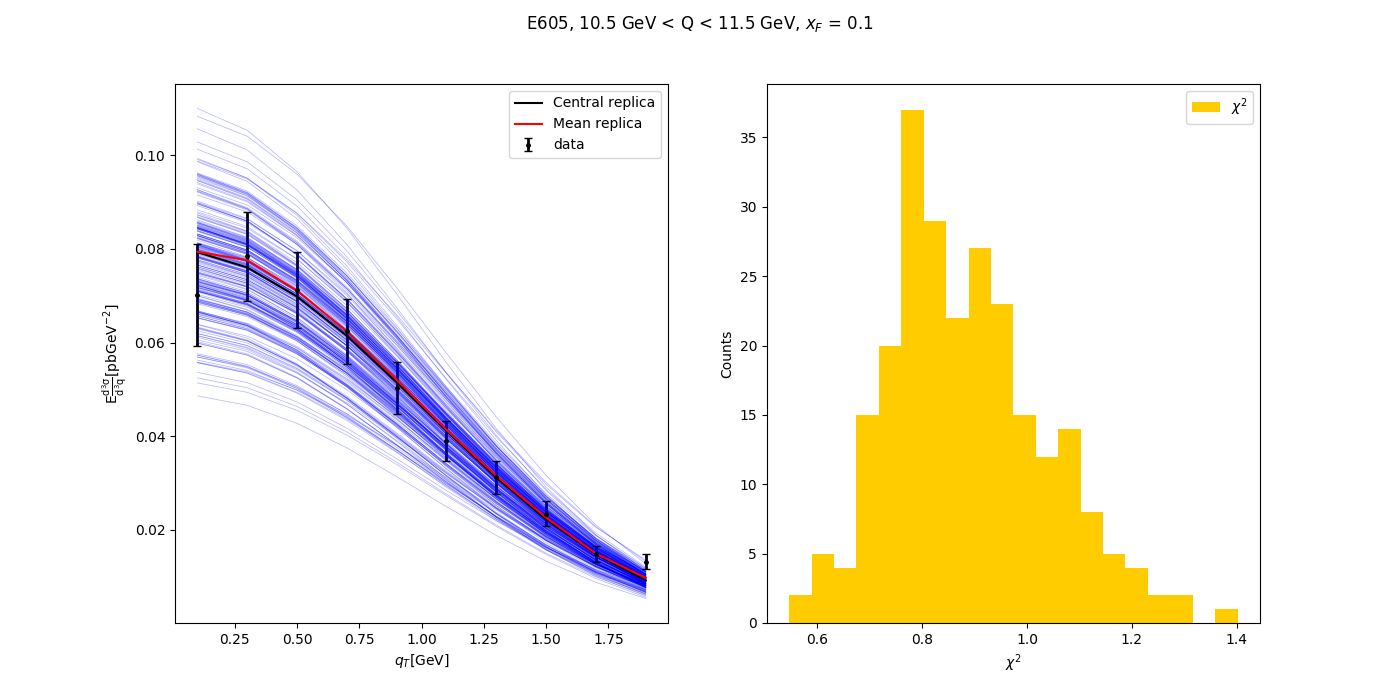
\includegraphics{pngplots/E605_Q_10.5_11.5.png}
\caption{E605\_Q\_10.5\_11.5 data-theory comparison}
\end{figure}

\begin{figure}
\centering
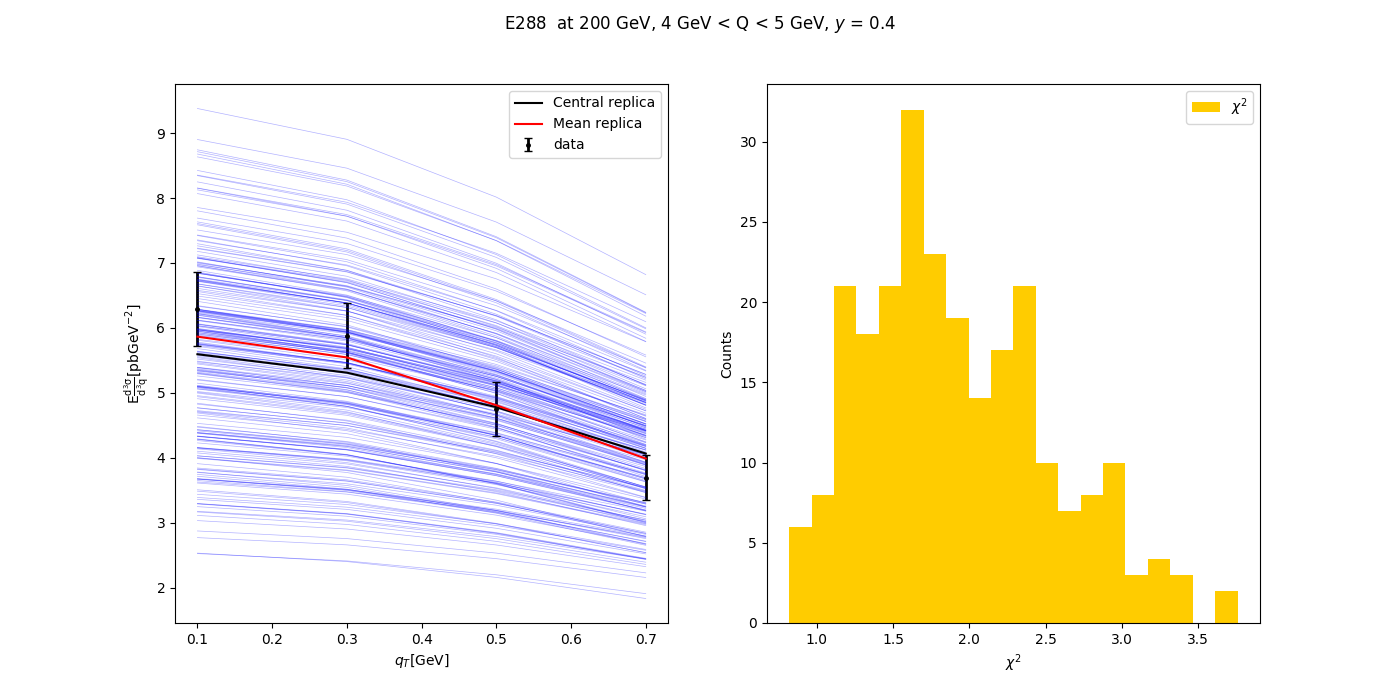
\includegraphics{pngplots/E288_200_Q_4_5.png}
\caption{E288\_200\_Q\_4\_5 data-theory comparison}
\end{figure}

\begin{figure}
\centering
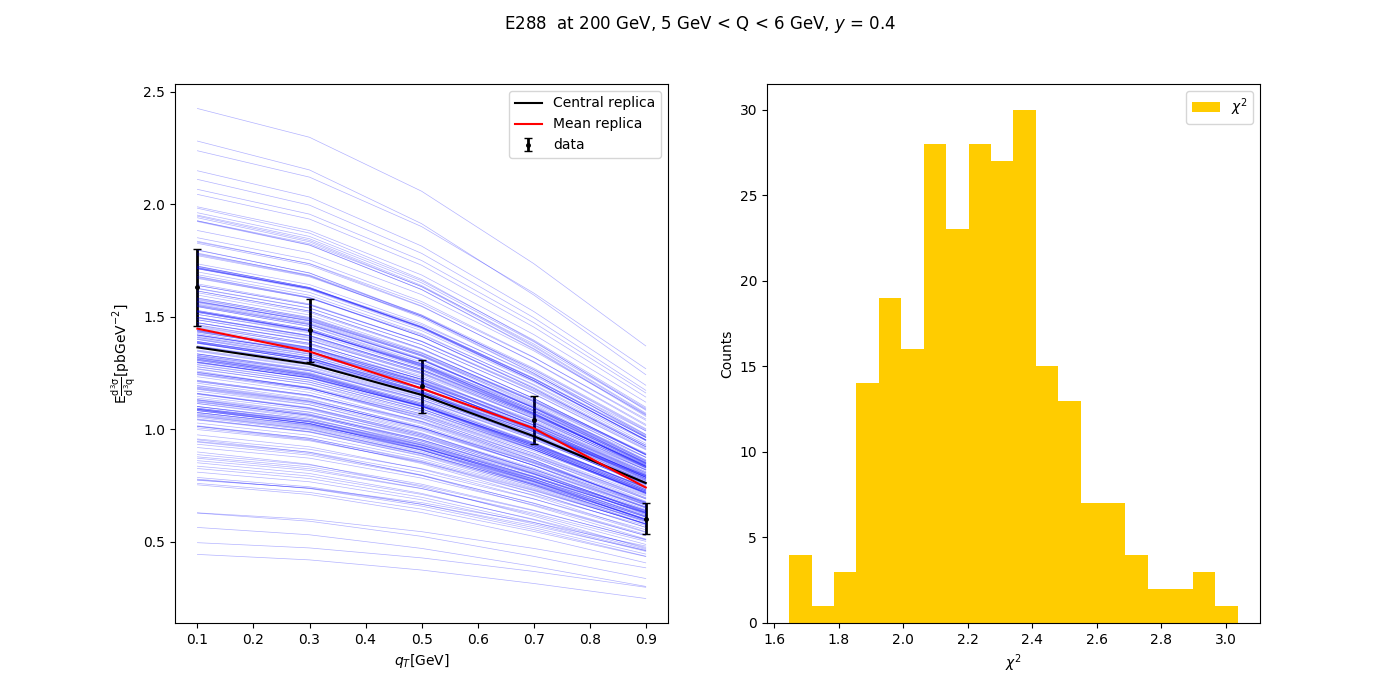
\includegraphics{pngplots/E288_200_Q_5_6.png}
\caption{E288\_200\_Q\_5\_6 data-theory comparison}
\end{figure}

\begin{figure}
\centering
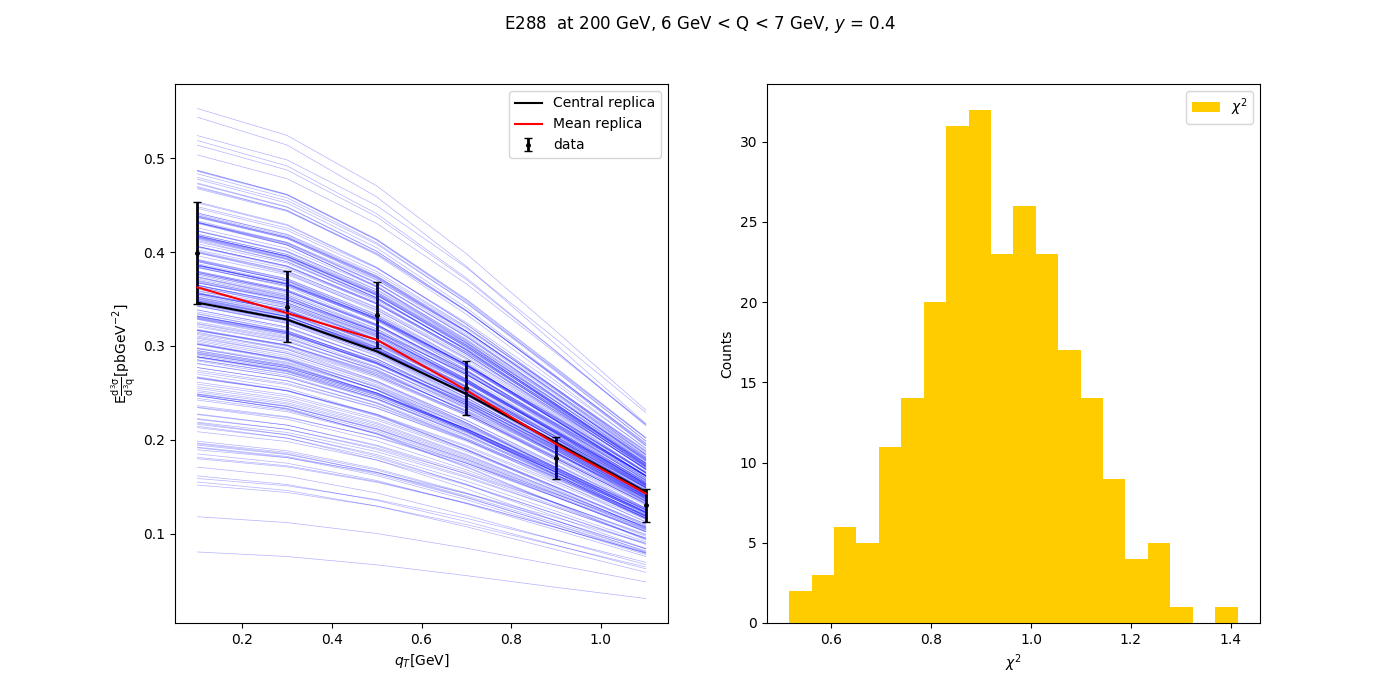
\includegraphics{pngplots/E288_200_Q_6_7.png}
\caption{E288\_200\_Q\_6\_7 data-theory comparison}
\end{figure}

\begin{figure}
\centering
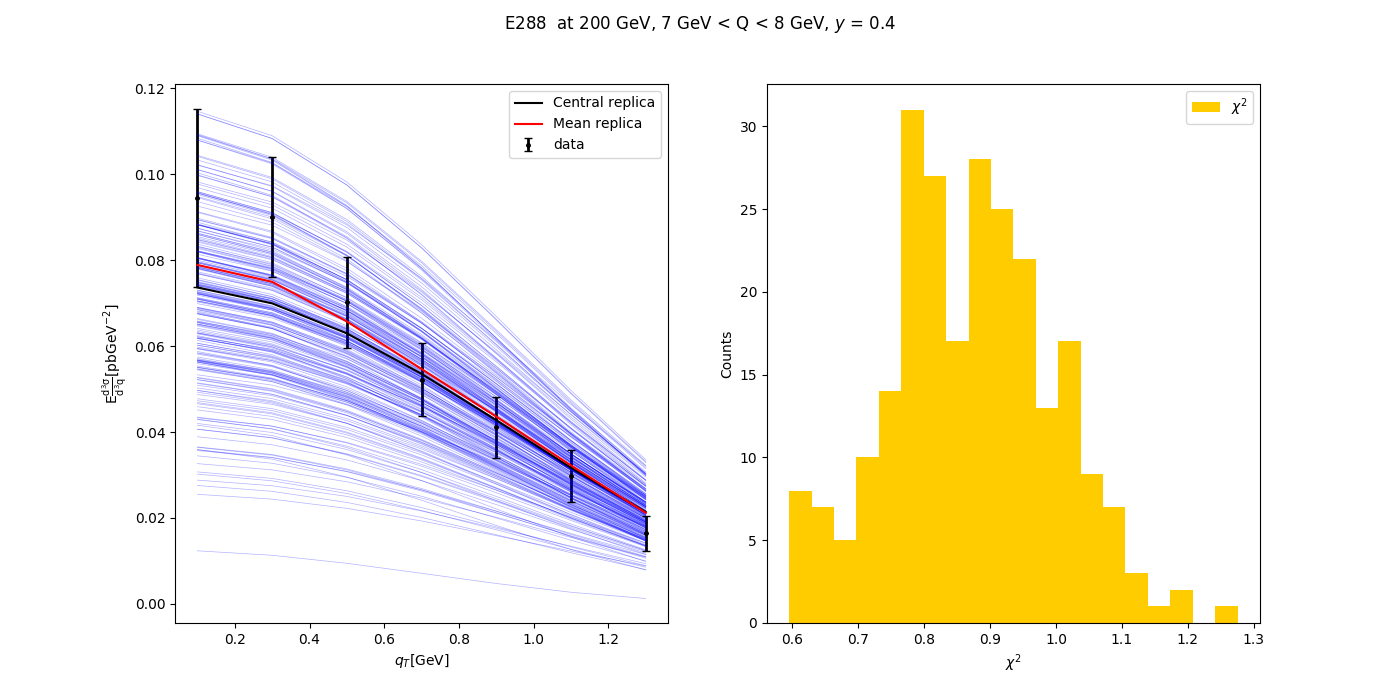
\includegraphics{pngplots/E288_200_Q_7_8.png}
\caption{E288\_200\_Q\_7\_8 data-theory comparison}
\end{figure}

\begin{figure}
\centering
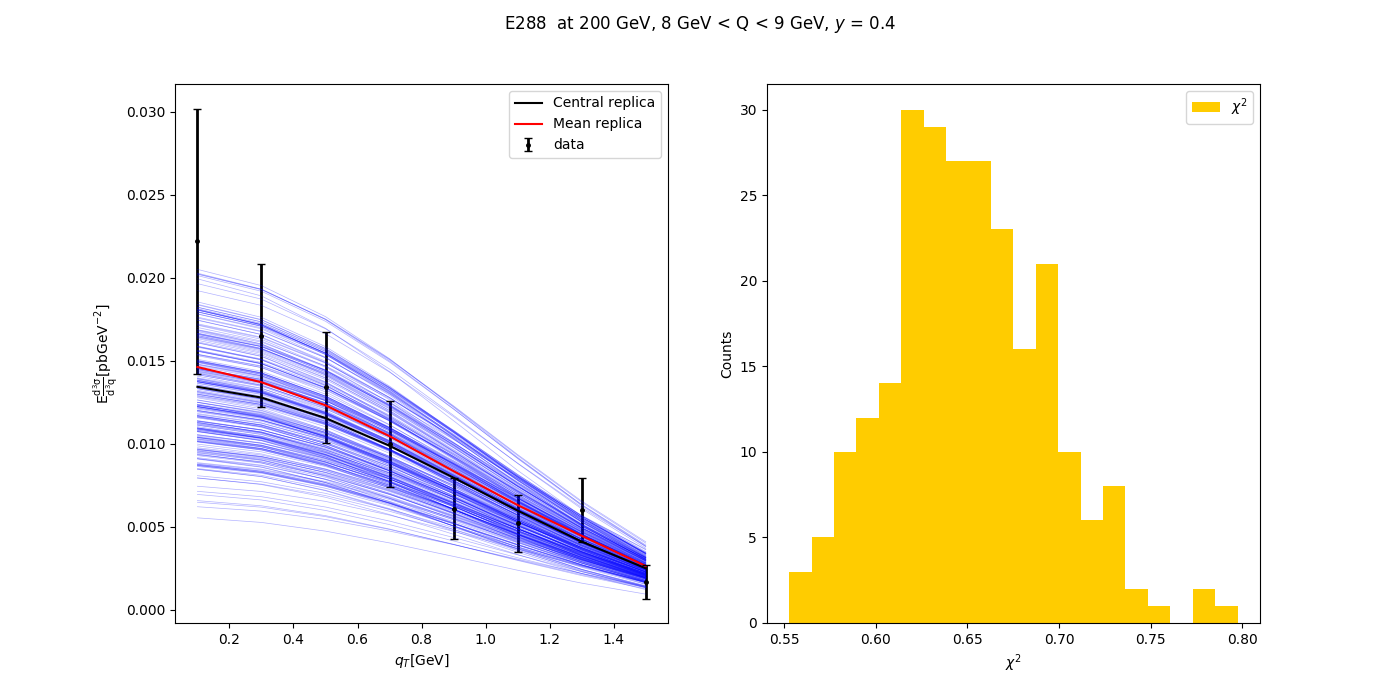
\includegraphics{pngplots/E288_200_Q_8_9.png}
\caption{E288\_200\_Q\_8\_9 data-theory comparison}
\end{figure}

\begin{figure}
\centering
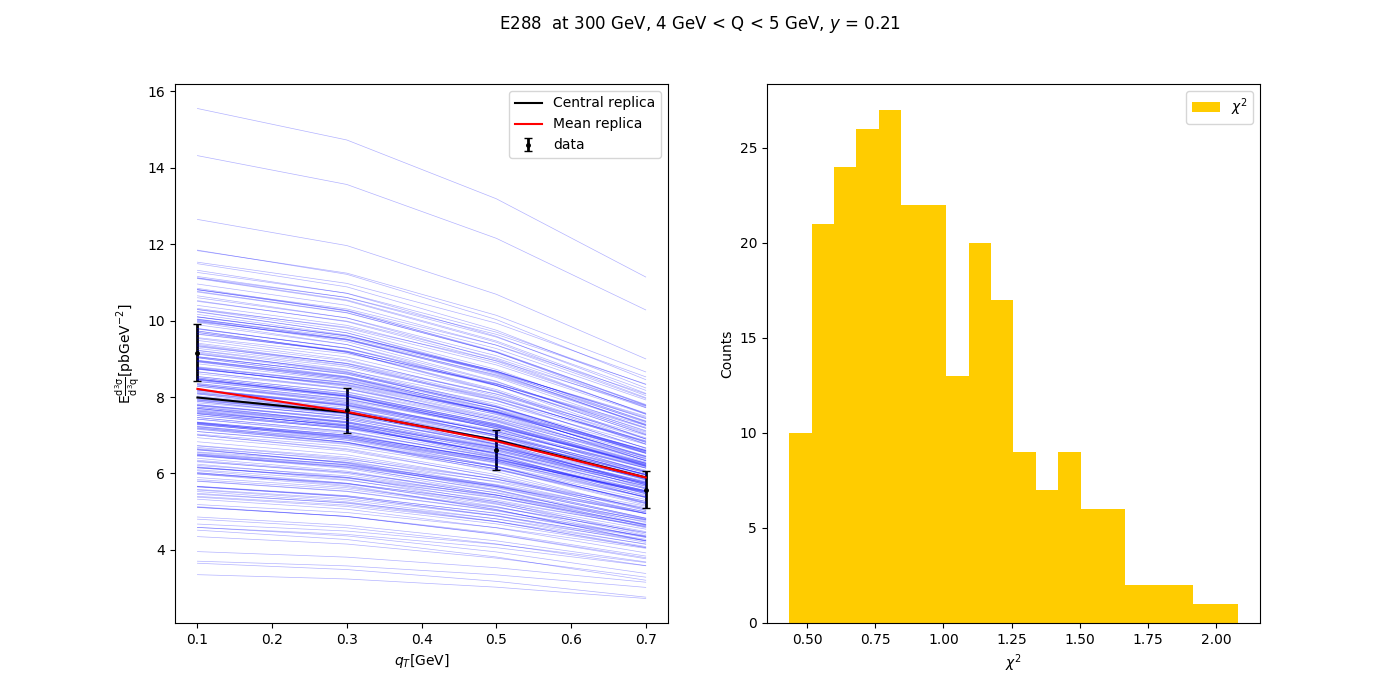
\includegraphics{pngplots/E288_300_Q_4_5.png}
\caption{E288\_300\_Q\_4\_5 data-theory comparison}
\end{figure}

\begin{figure}
\centering
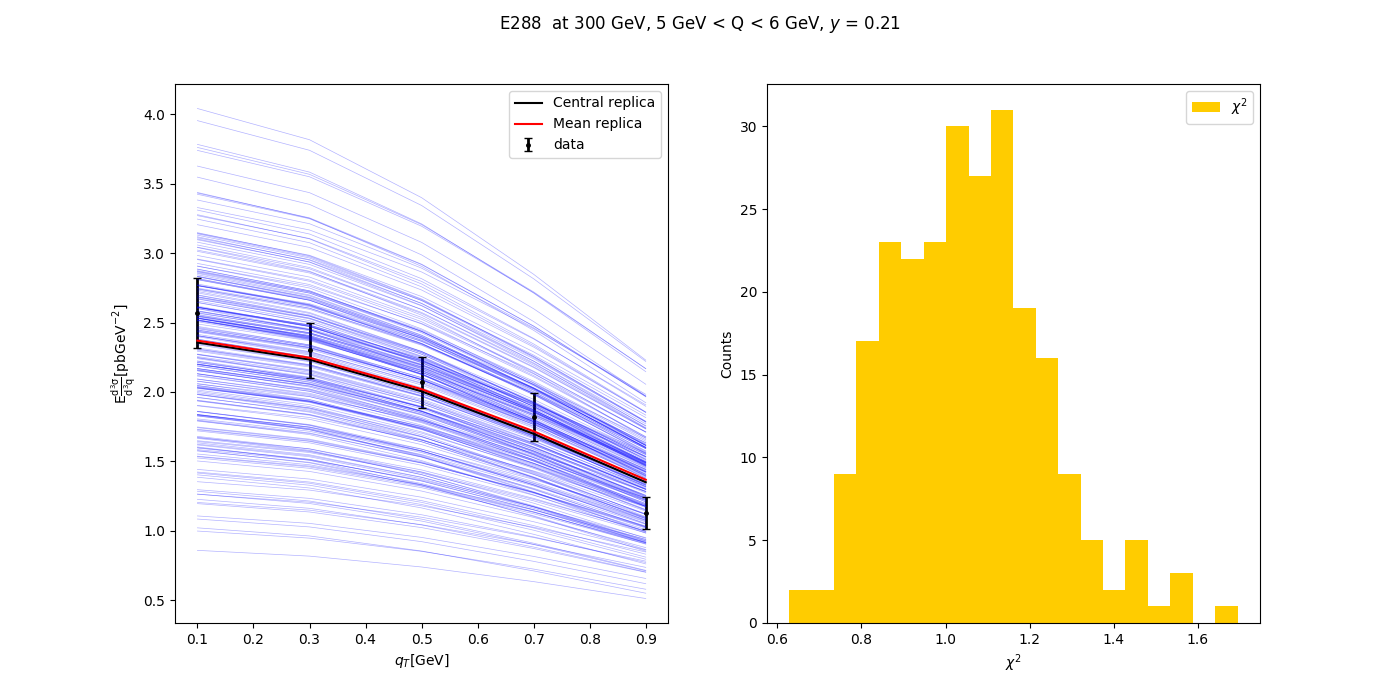
\includegraphics{pngplots/E288_300_Q_5_6.png}
\caption{E288\_300\_Q\_5\_6 data-theory comparison}
\end{figure}

\begin{figure}
\centering
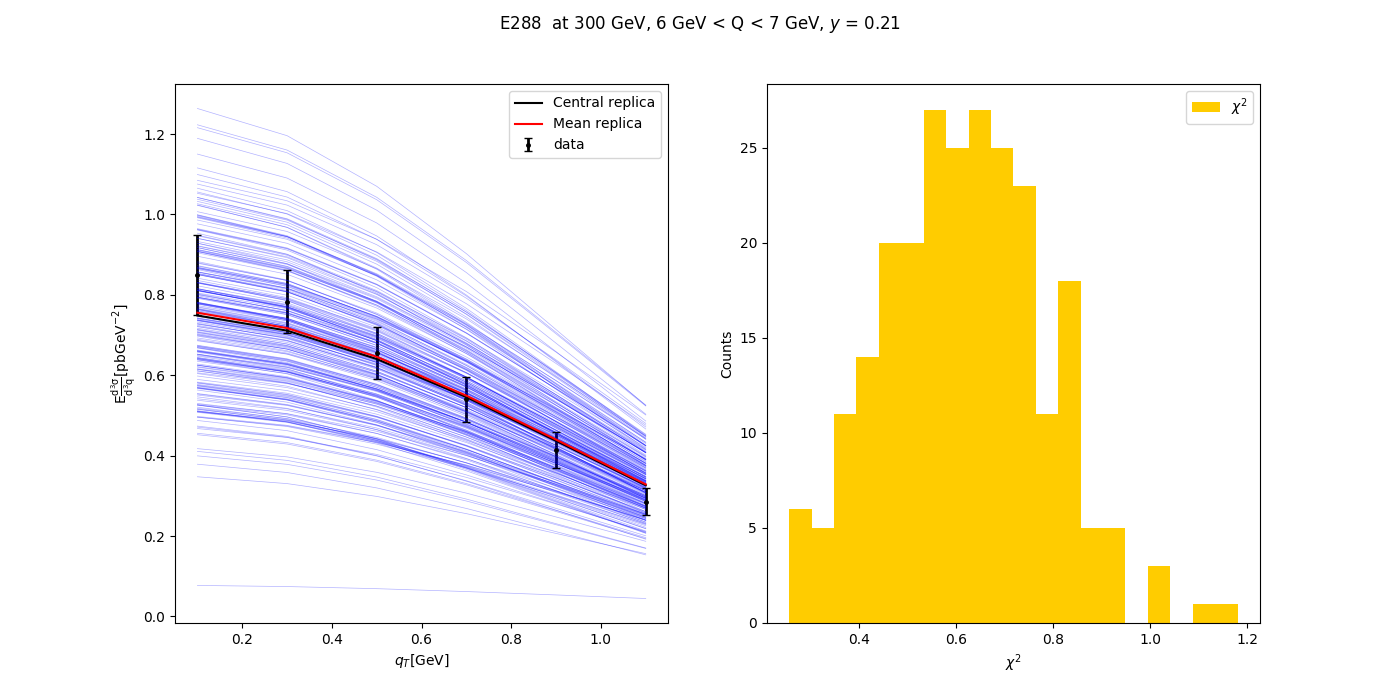
\includegraphics{pngplots/E288_300_Q_6_7.png}
\caption{E288\_300\_Q\_6\_7 data-theory comparison}
\end{figure}

\begin{figure}
\centering
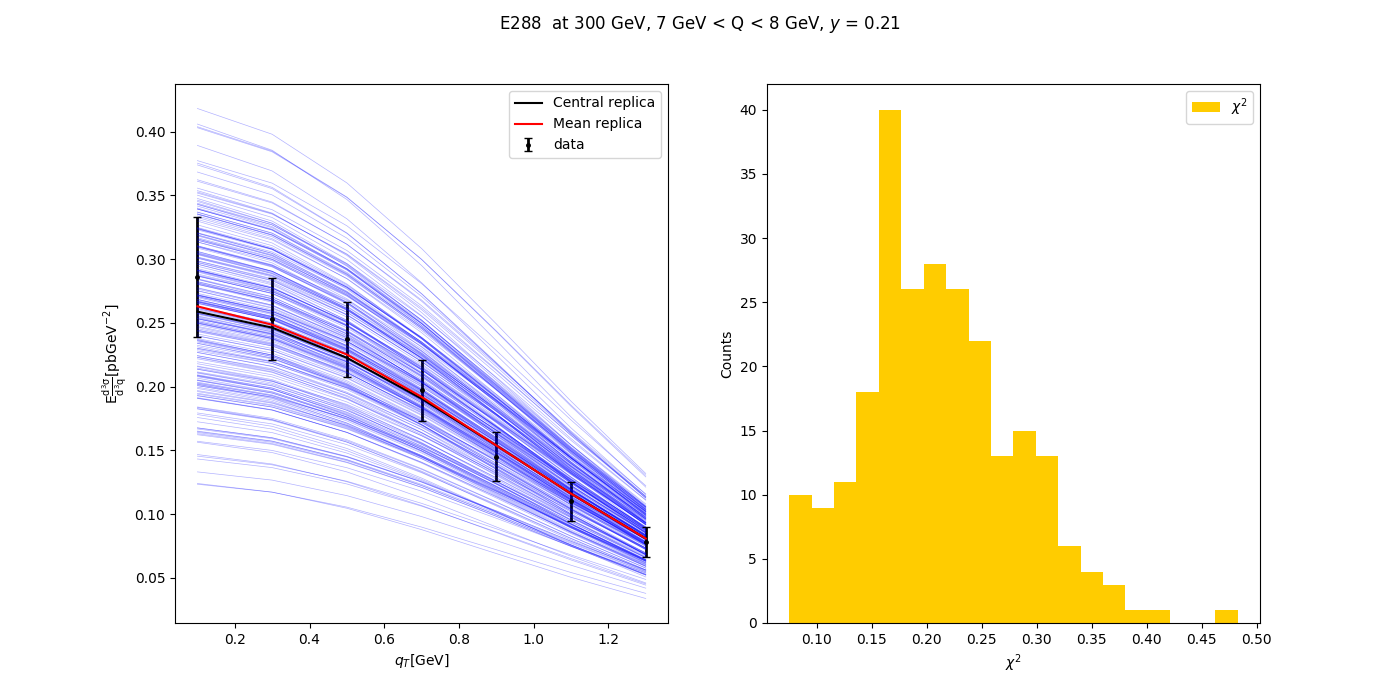
\includegraphics{pngplots/E288_300_Q_7_8.png}
\caption{E288\_300\_Q\_7\_8 data-theory comparison}
\end{figure}

\begin{figure}
\centering
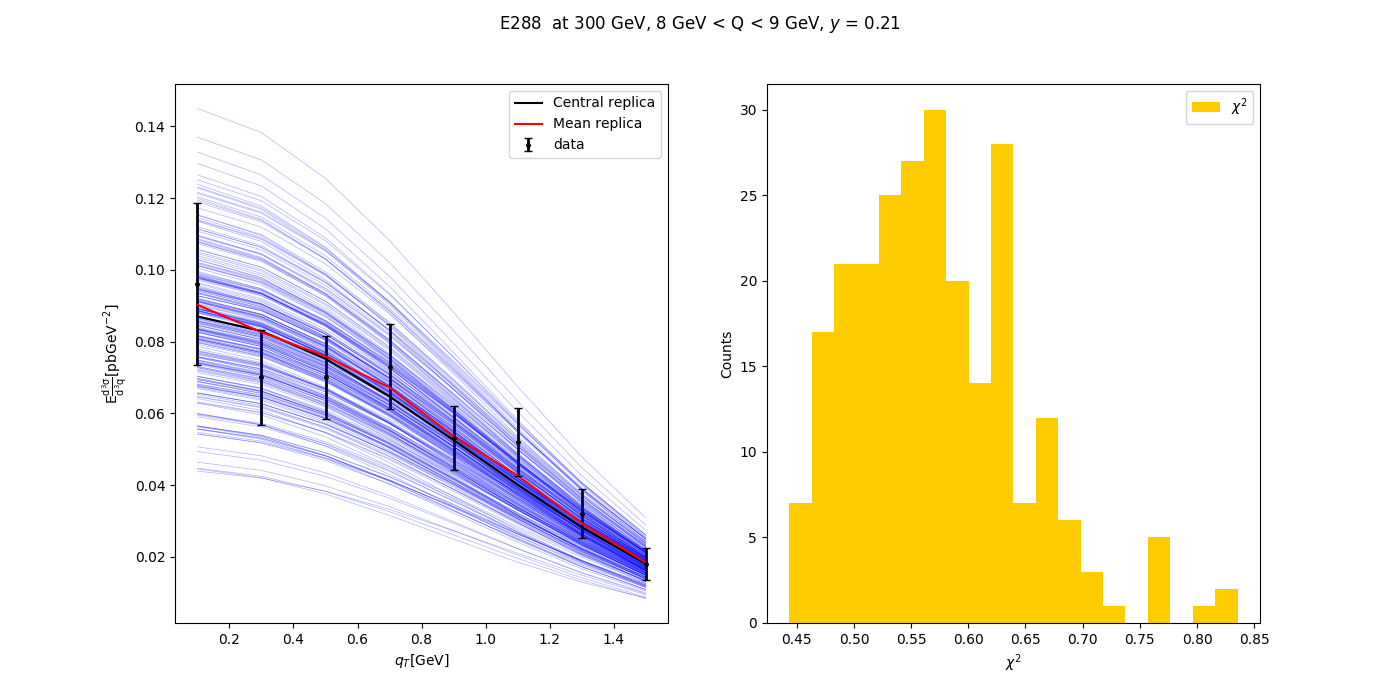
\includegraphics{pngplots/E288_300_Q_8_9.png}
\caption{E288\_300\_Q\_8\_9 data-theory comparison}
\end{figure}

\begin{figure}
\centering
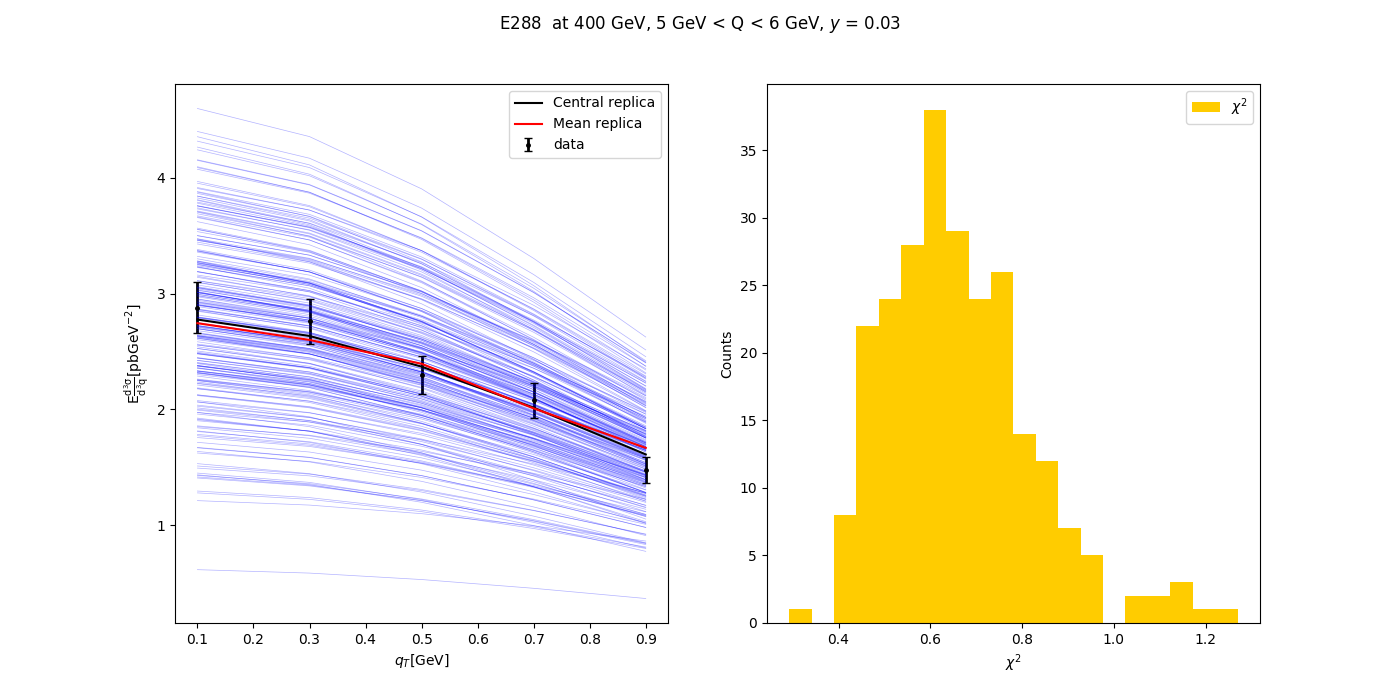
\includegraphics{pngplots/E288_400_Q_5_6.png}
\caption{E288\_400\_Q\_5\_6 data-theory comparison}
\end{figure}

\begin{figure}
\centering
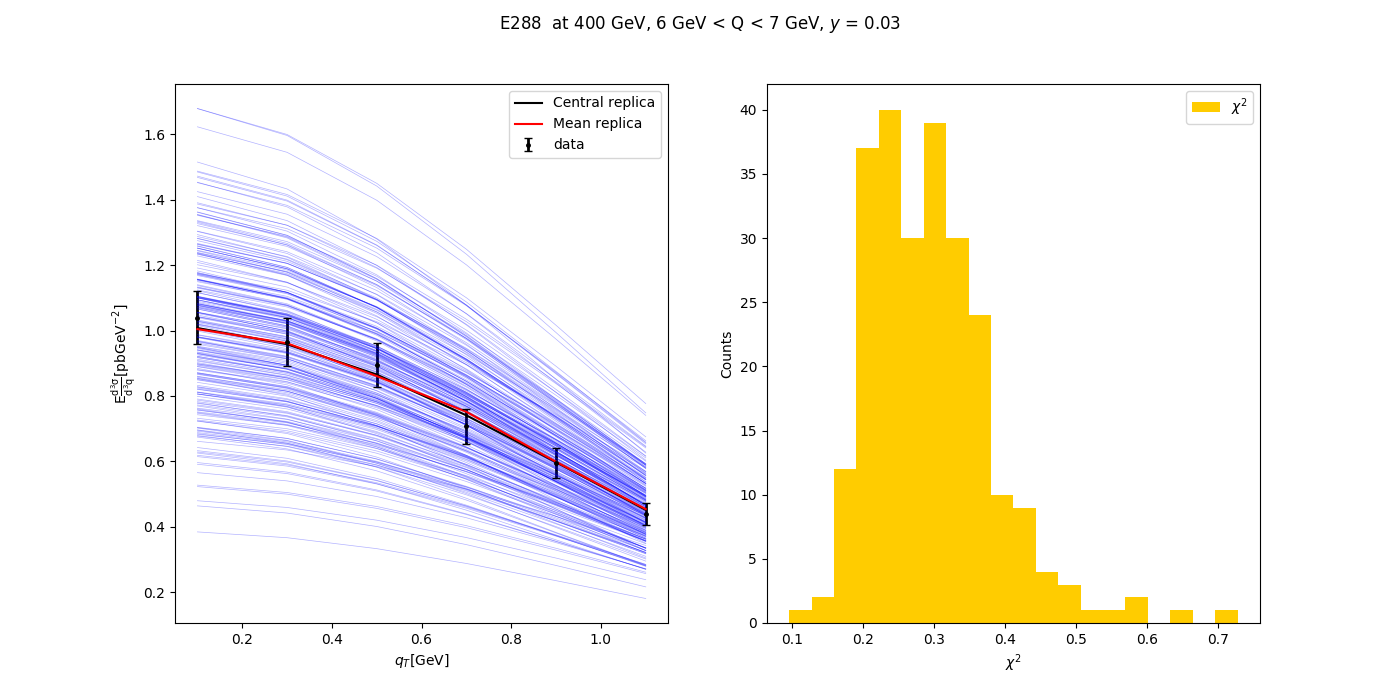
\includegraphics{pngplots/E288_400_Q_6_7.png}
\caption{E288\_400\_Q\_6\_7 data-theory comparison}
\end{figure}

\begin{figure}
\centering
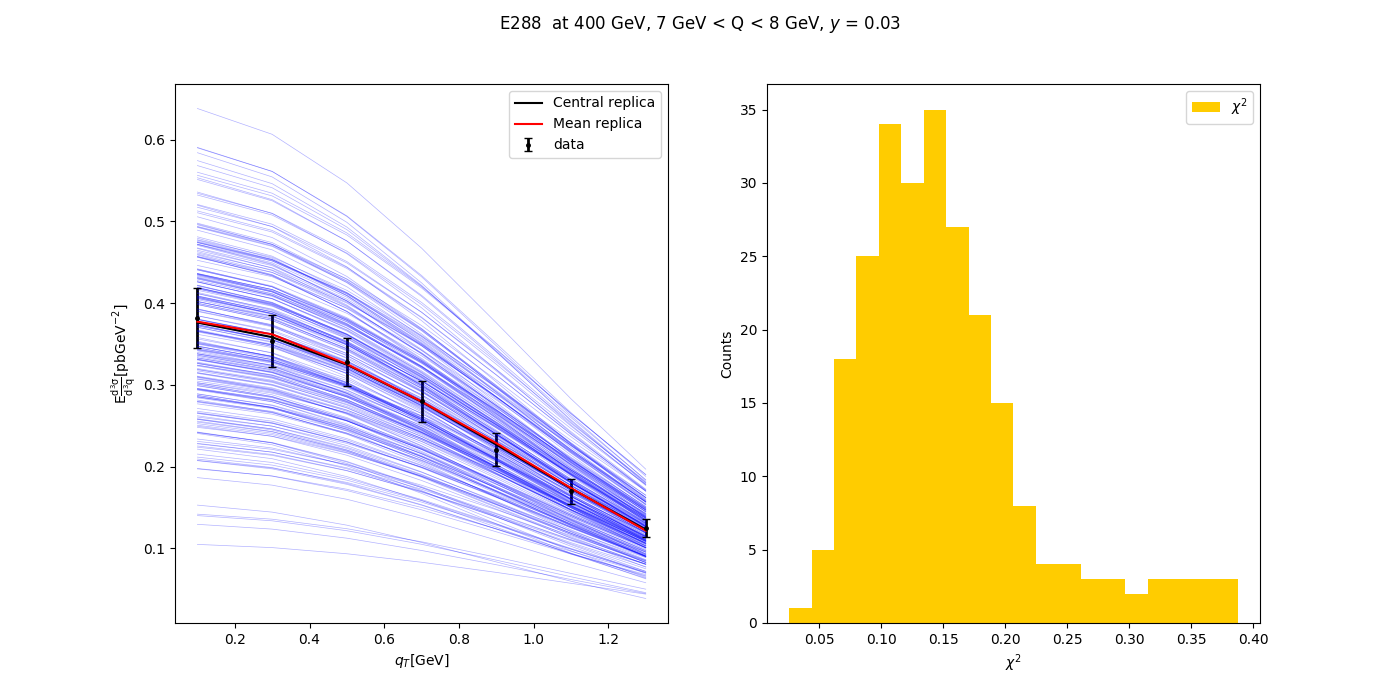
\includegraphics{pngplots/E288_400_Q_7_8.png}
\caption{E288\_400\_Q\_7\_8 data-theory comparison}
\end{figure}

\begin{figure}
\centering
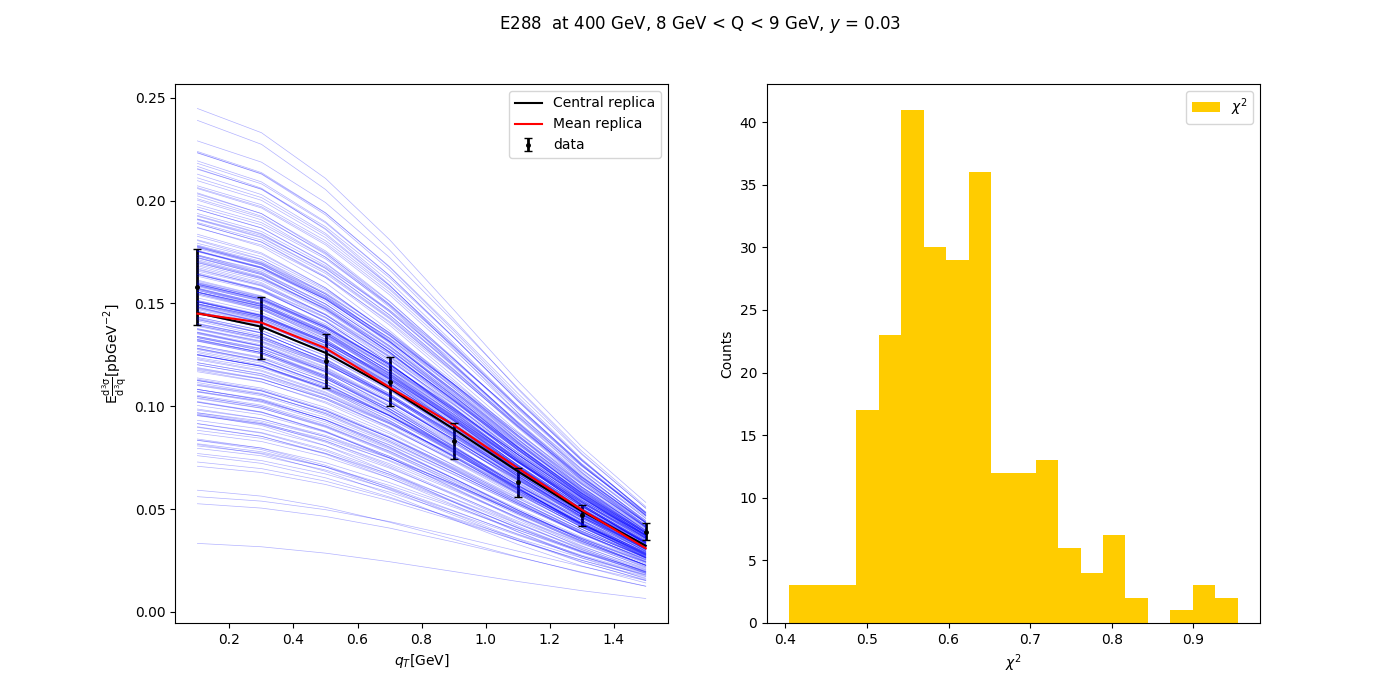
\includegraphics{pngplots/E288_400_Q_8_9.png}
\caption{E288\_400\_Q\_8\_9 data-theory comparison}
\end{figure}

\begin{figure}
\centering
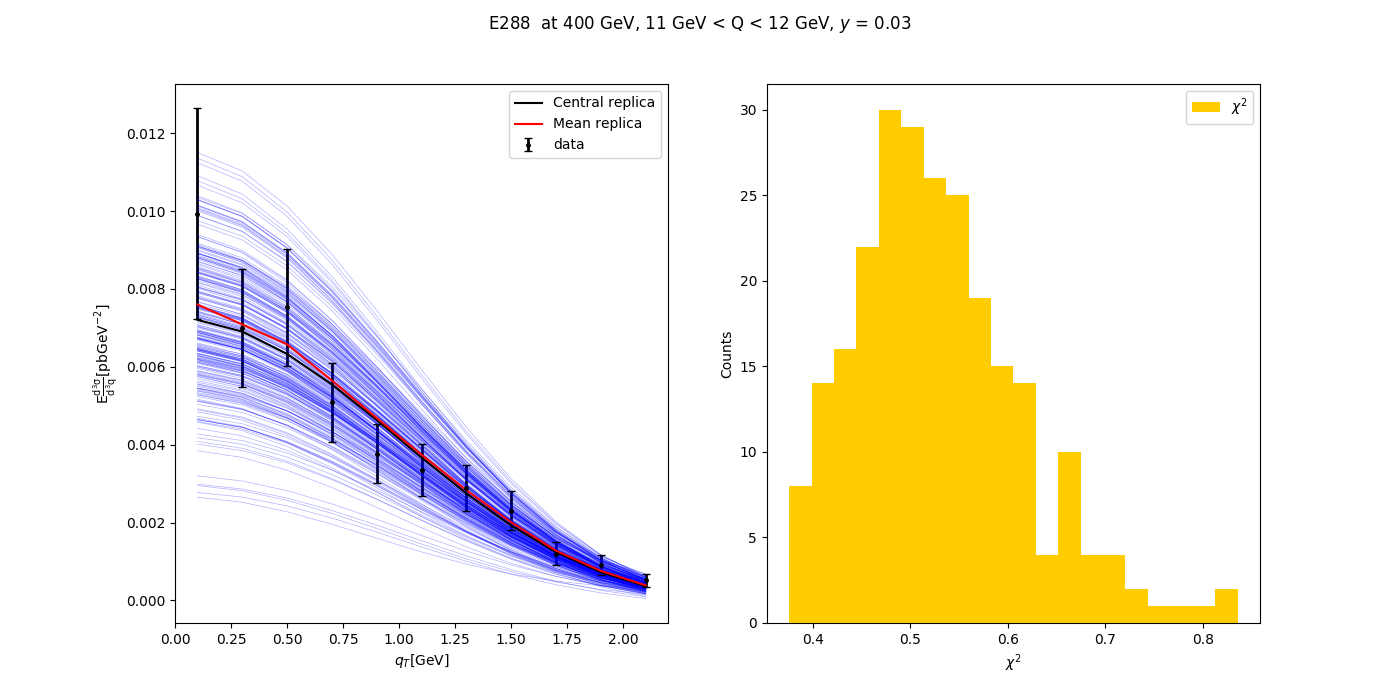
\includegraphics{pngplots/E288_400_Q_11_12.png}
\caption{E288\_400\_Q\_11\_12 data-theory comparison}
\end{figure}

\begin{figure}
\centering
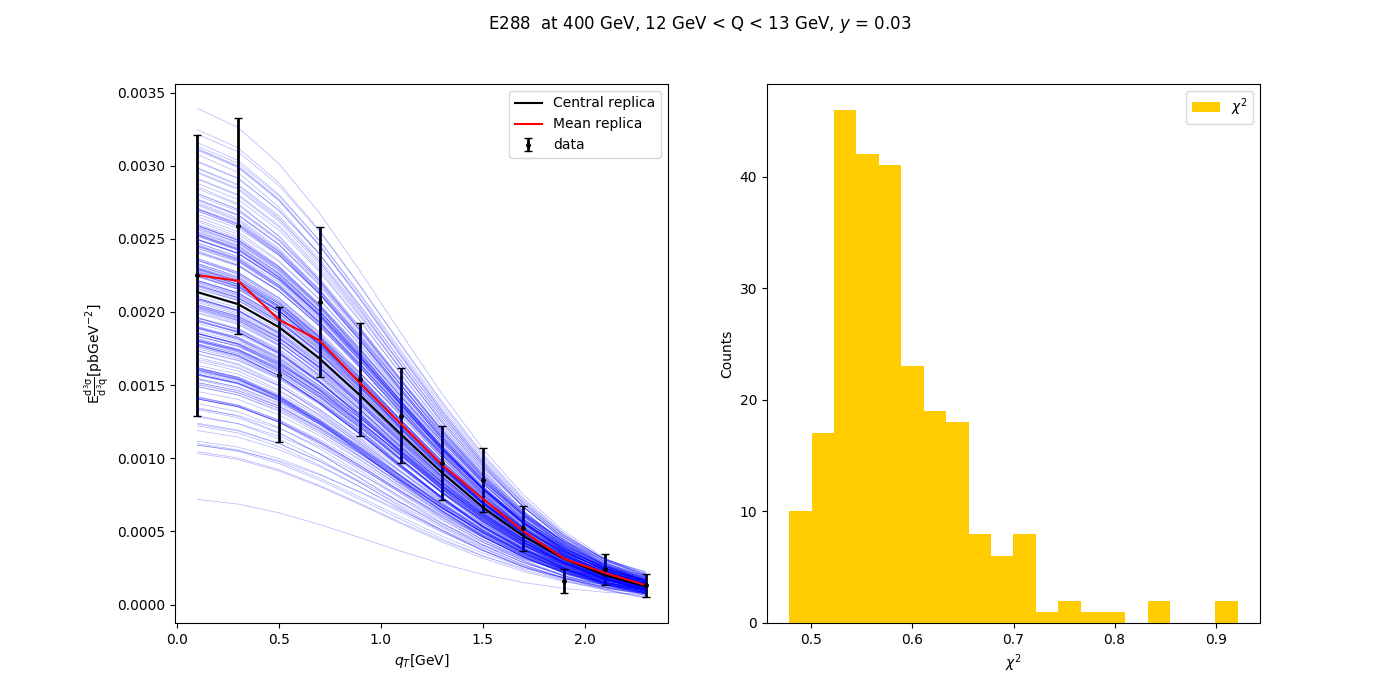
\includegraphics{pngplots/E288_400_Q_12_13.png}
\caption{E288\_400\_Q\_12\_13 data-theory comparison}
\end{figure}

\begin{figure}
\centering
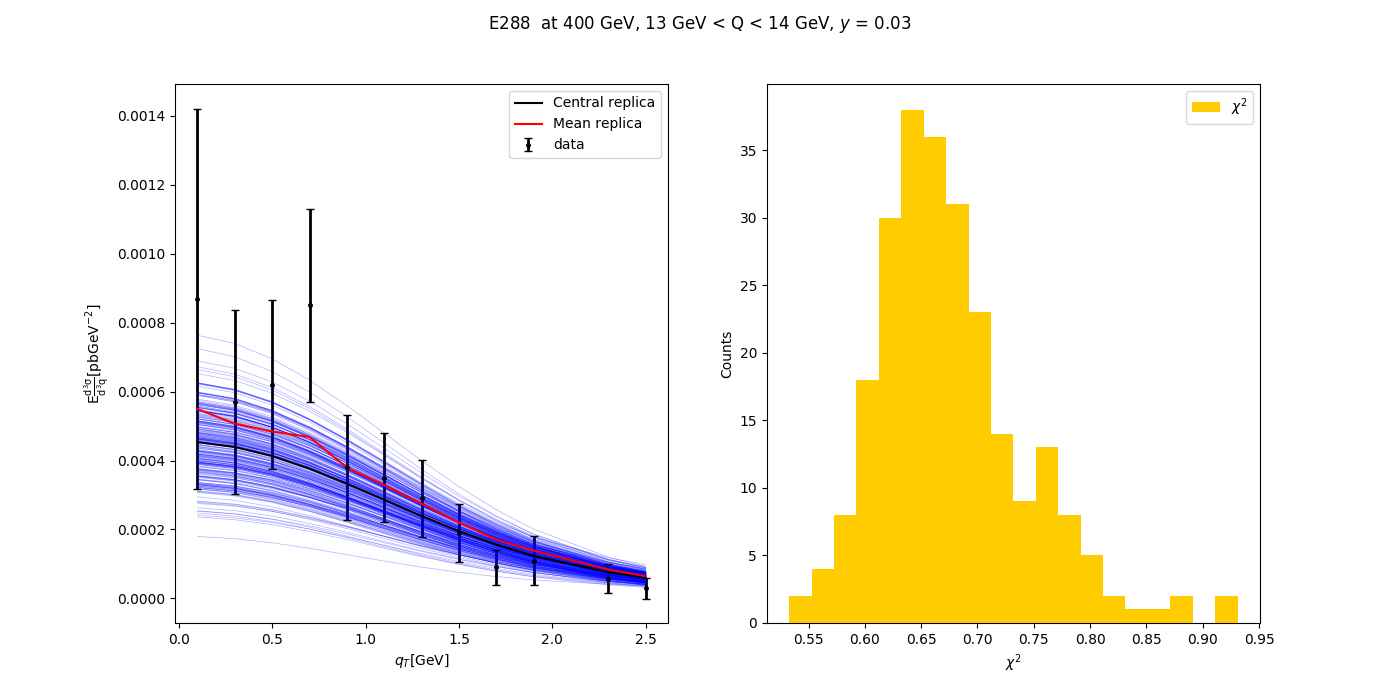
\includegraphics{pngplots/E288_400_Q_13_14.png}
\caption{E288\_400\_Q\_13\_14 data-theory comparison}
\end{figure}

\begin{figure}
\centering
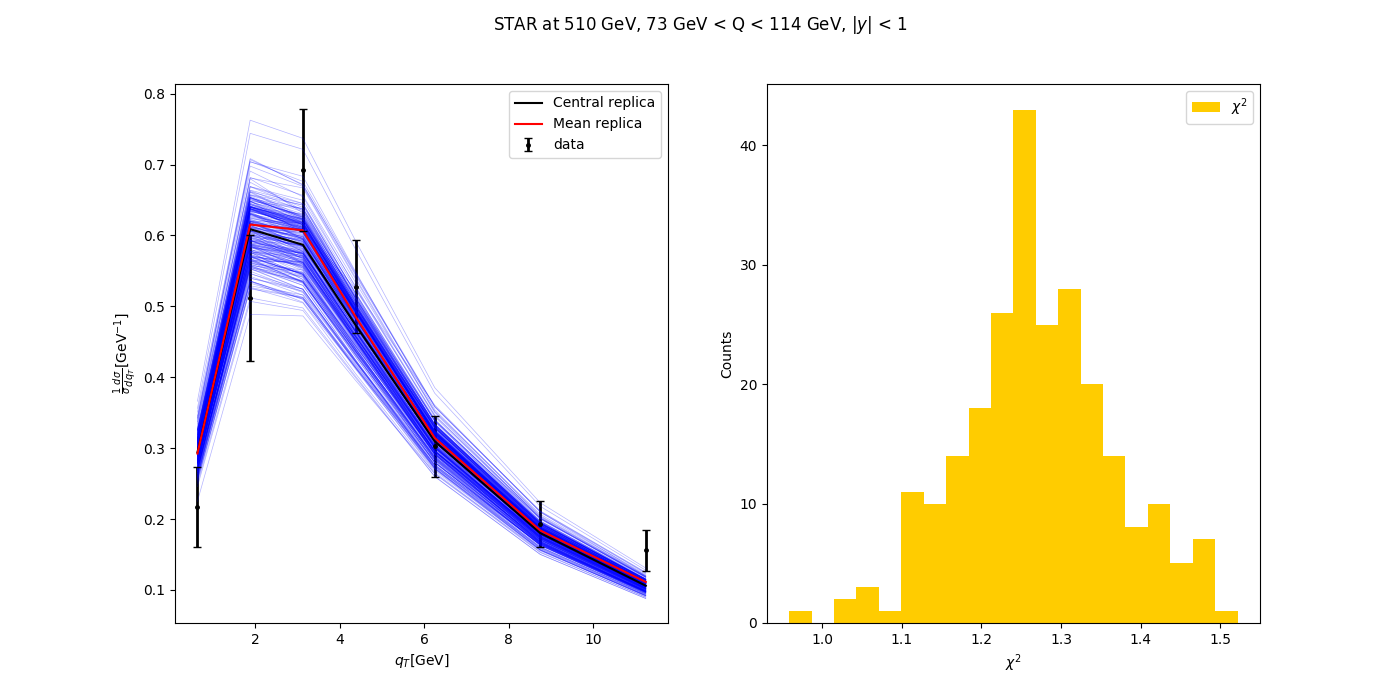
\includegraphics{pngplots/STAR_510.png}
\caption{STAR\_510 data-theory comparison}
\end{figure}

\begin{figure}
\centering
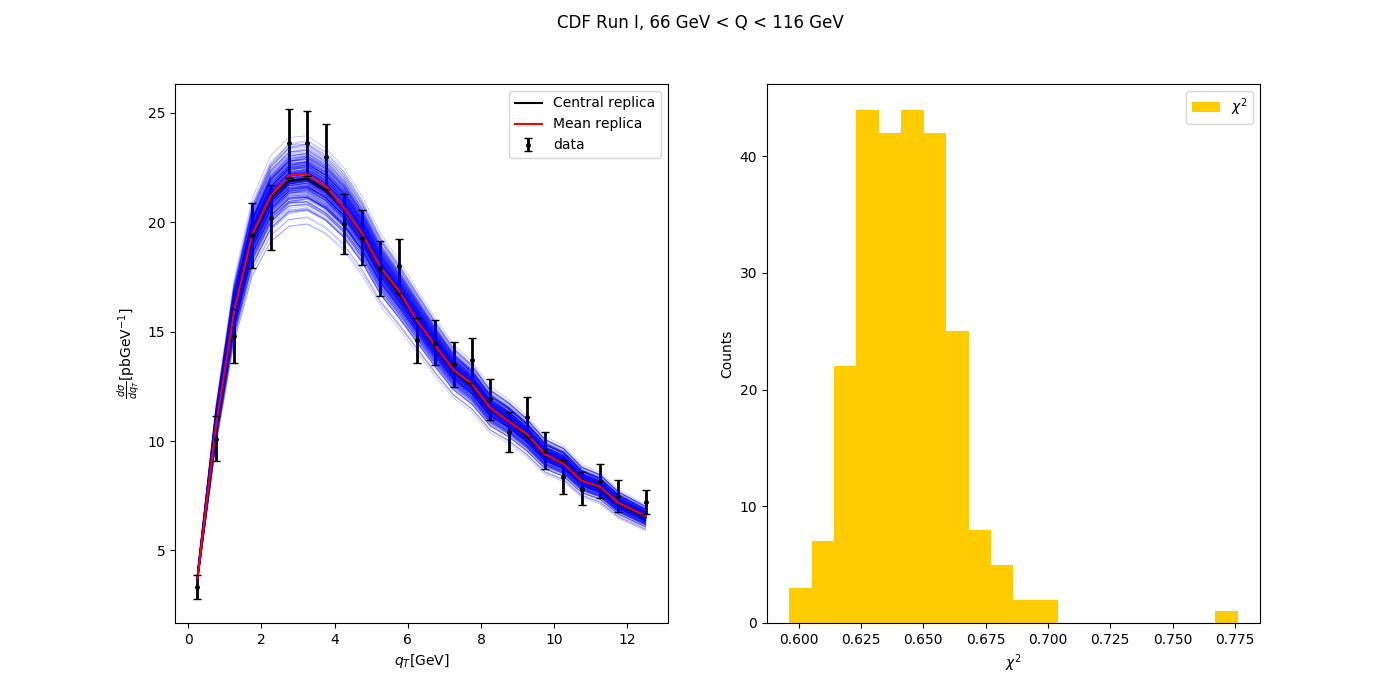
\includegraphics{pngplots/CDF_RunI.png}
\caption{CDF\_RunI data-theory comparison}
\end{figure}

\begin{figure}
\centering
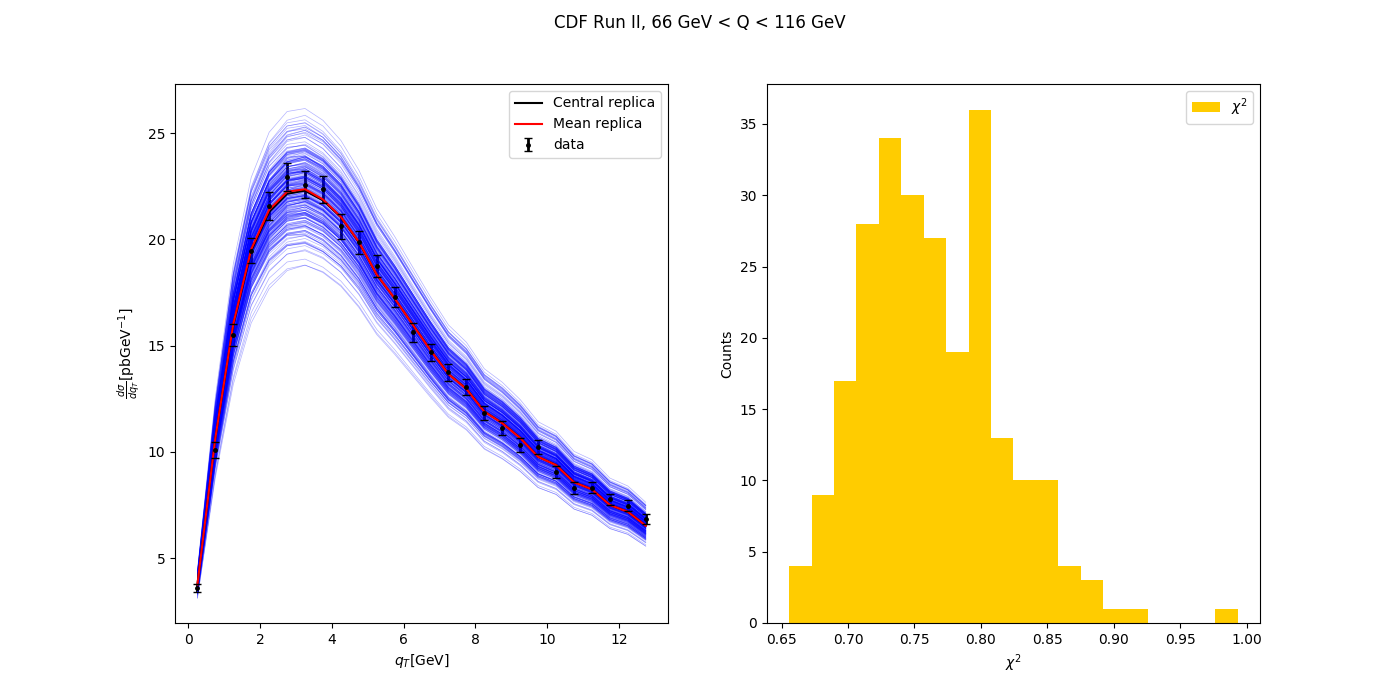
\includegraphics{pngplots/CDF_RunII.png}
\caption{CDF\_RunII data-theory comparison}
\end{figure}

\begin{figure}
\centering
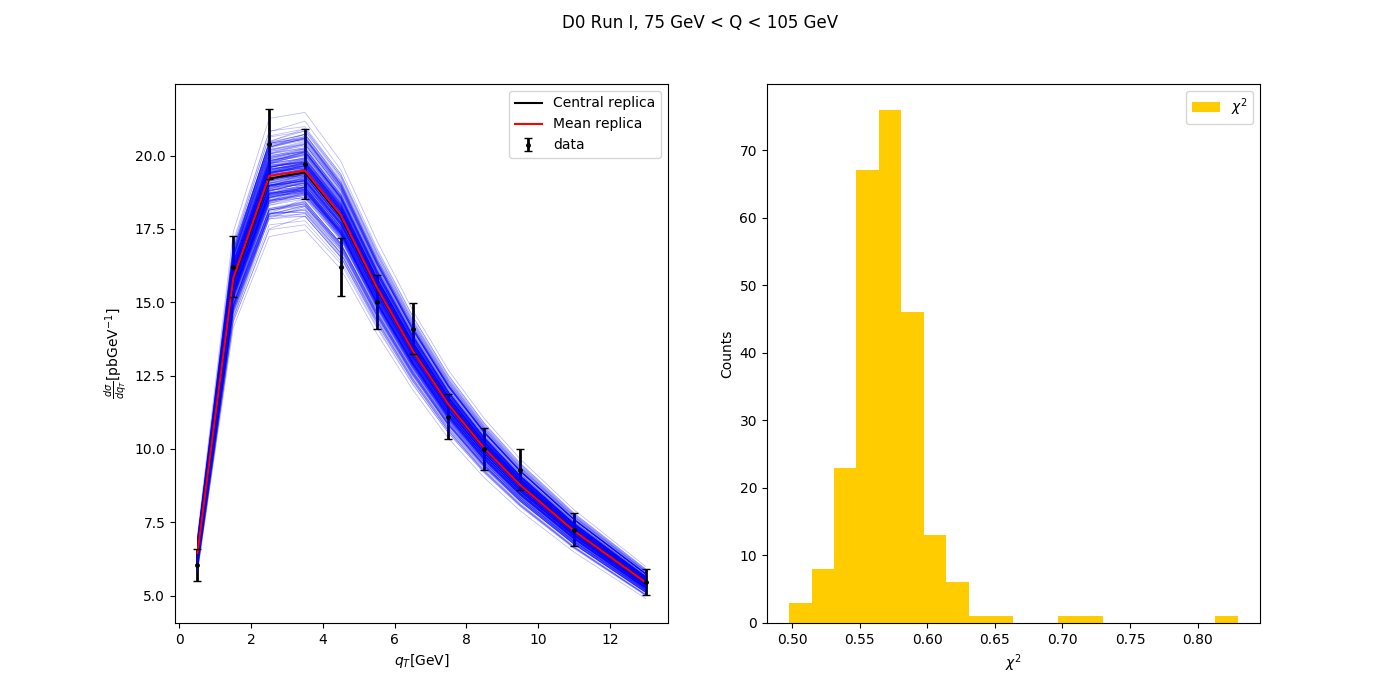
\includegraphics{pngplots/D0_RunI.png}
\caption{D0\_RunI data-theory comparison}
\end{figure}

\begin{figure}
\centering
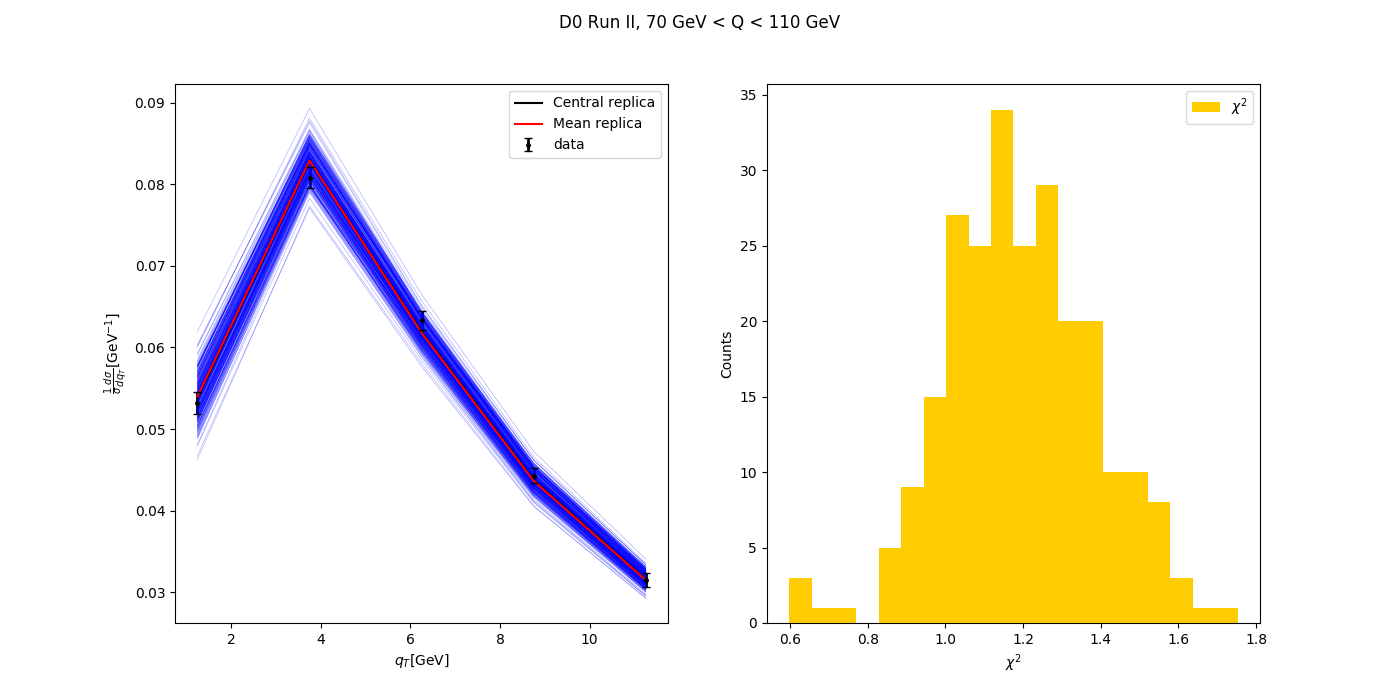
\includegraphics{pngplots/D0_RunII.png}
\caption{D0\_RunII data-theory comparison}
\end{figure}

\begin{figure}
\centering
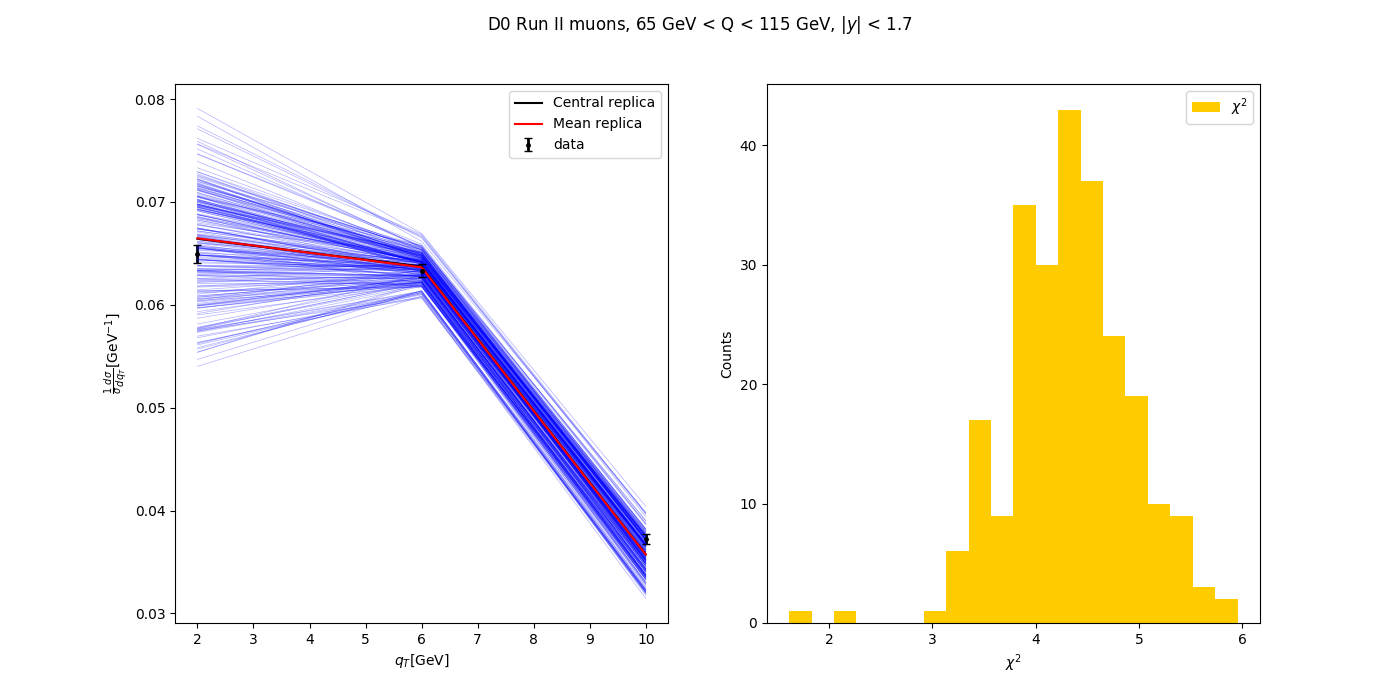
\includegraphics{pngplots/D0_RunIImu.png}
\caption{D0\_RunIImu data-theory comparison}
\end{figure}

\begin{figure}
\centering
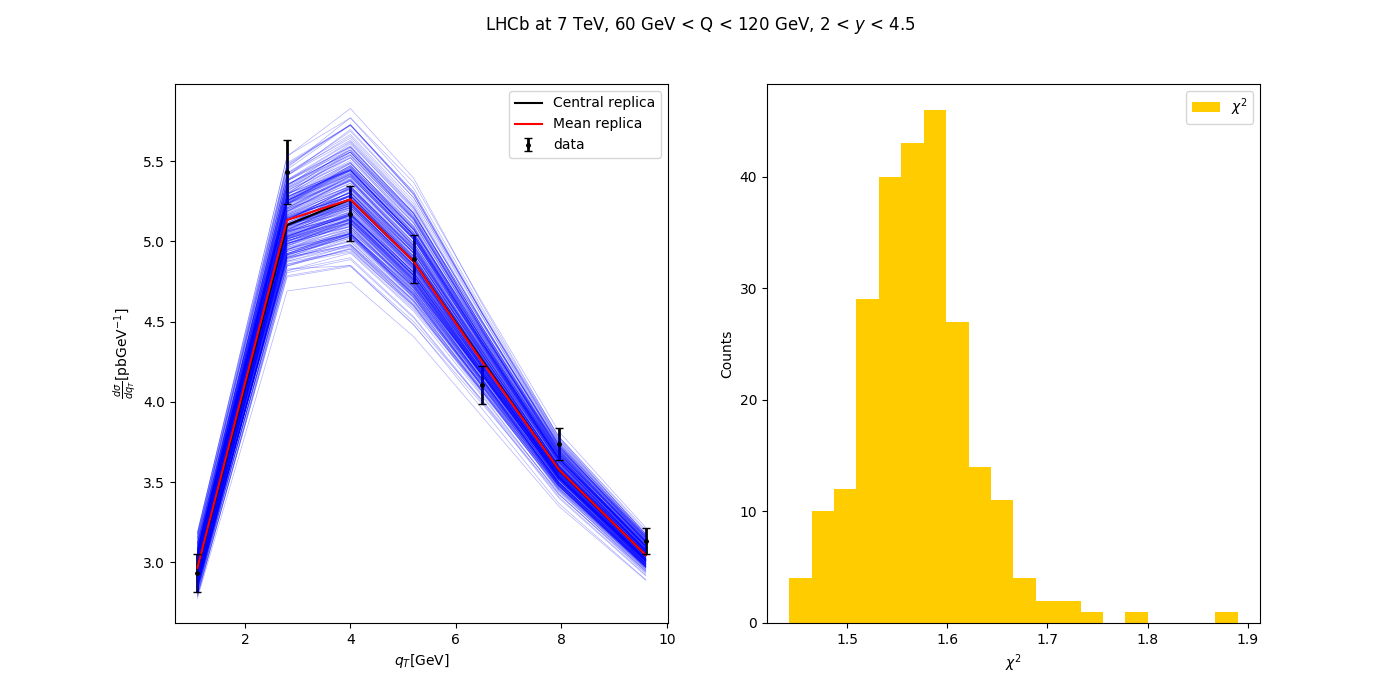
\includegraphics{pngplots/LHCb_7TeV.png}
\caption{LHCb\_7TeV data-theory comparison}
\end{figure}

\begin{figure}
\centering
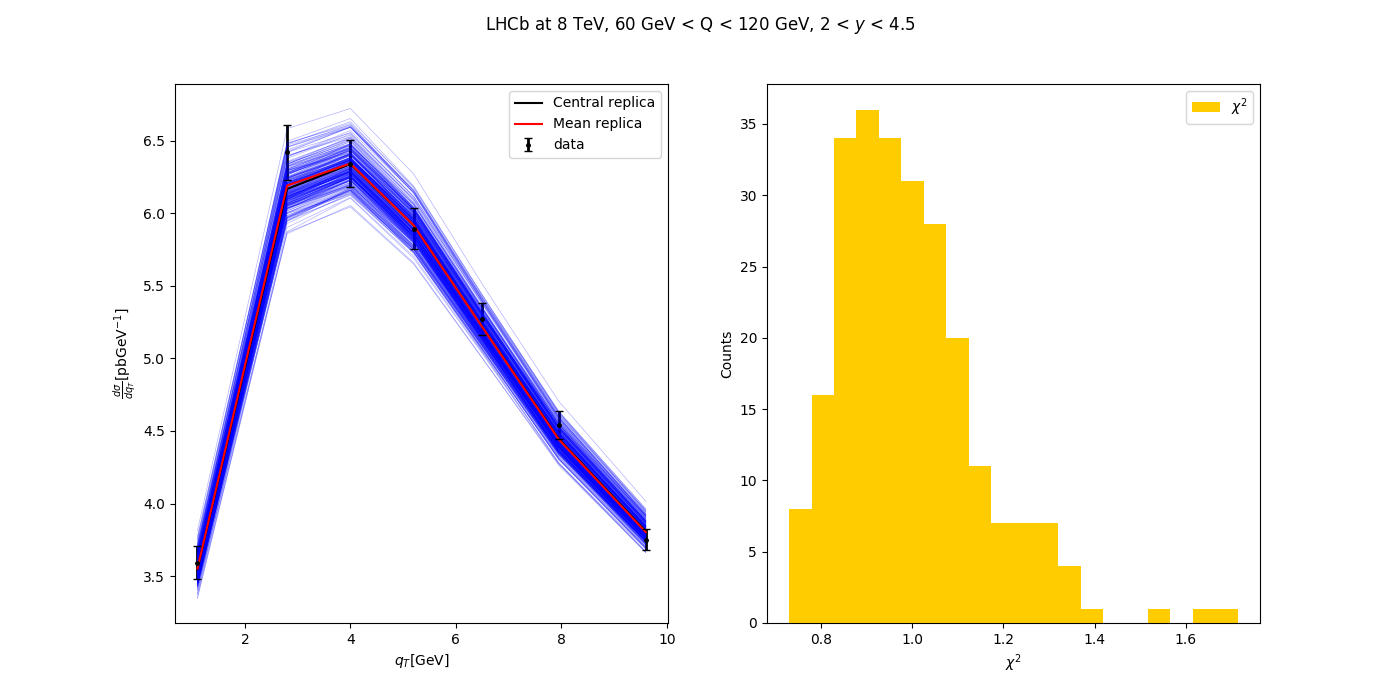
\includegraphics{pngplots/LHCb_8TeV.png}
\caption{LHCb\_8TeV data-theory comparison}
\end{figure}

\begin{figure}
\centering
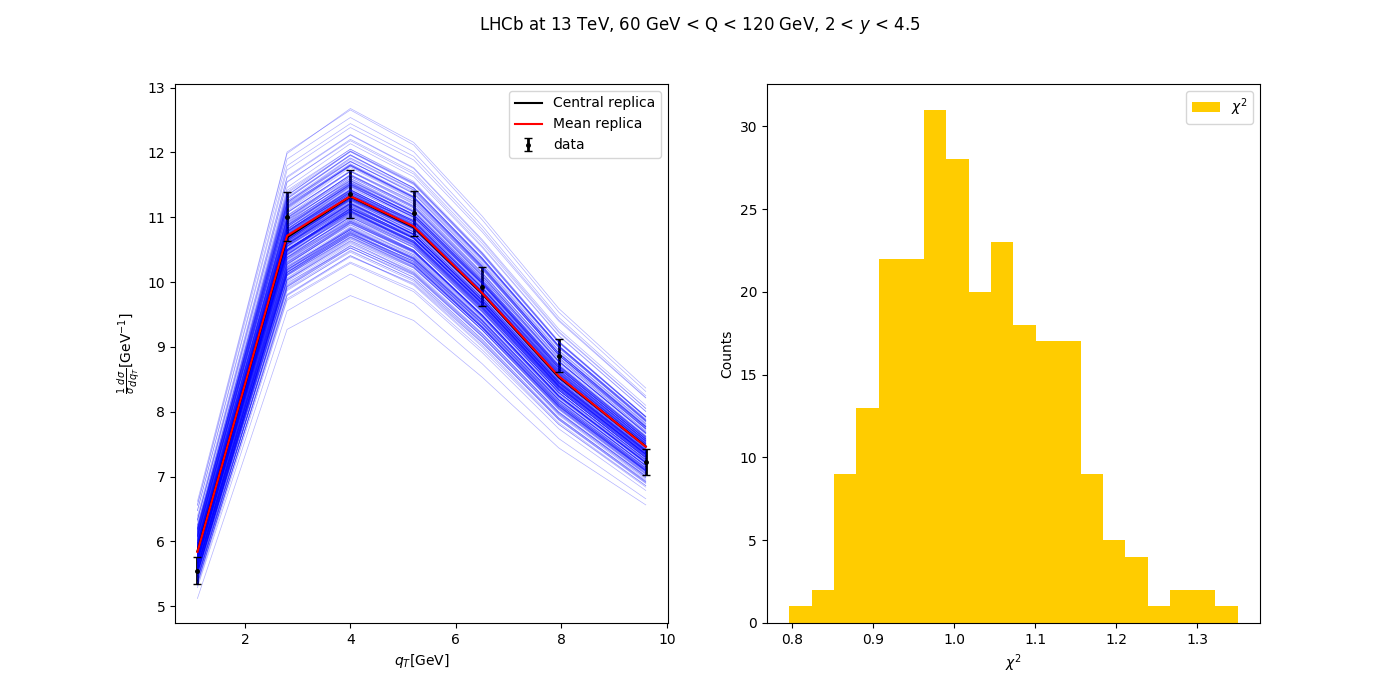
\includegraphics{pngplots/LHCb_13TeV.png}
\caption{LHCb\_13TeV data-theory comparison}
\end{figure}

\begin{figure}
\centering
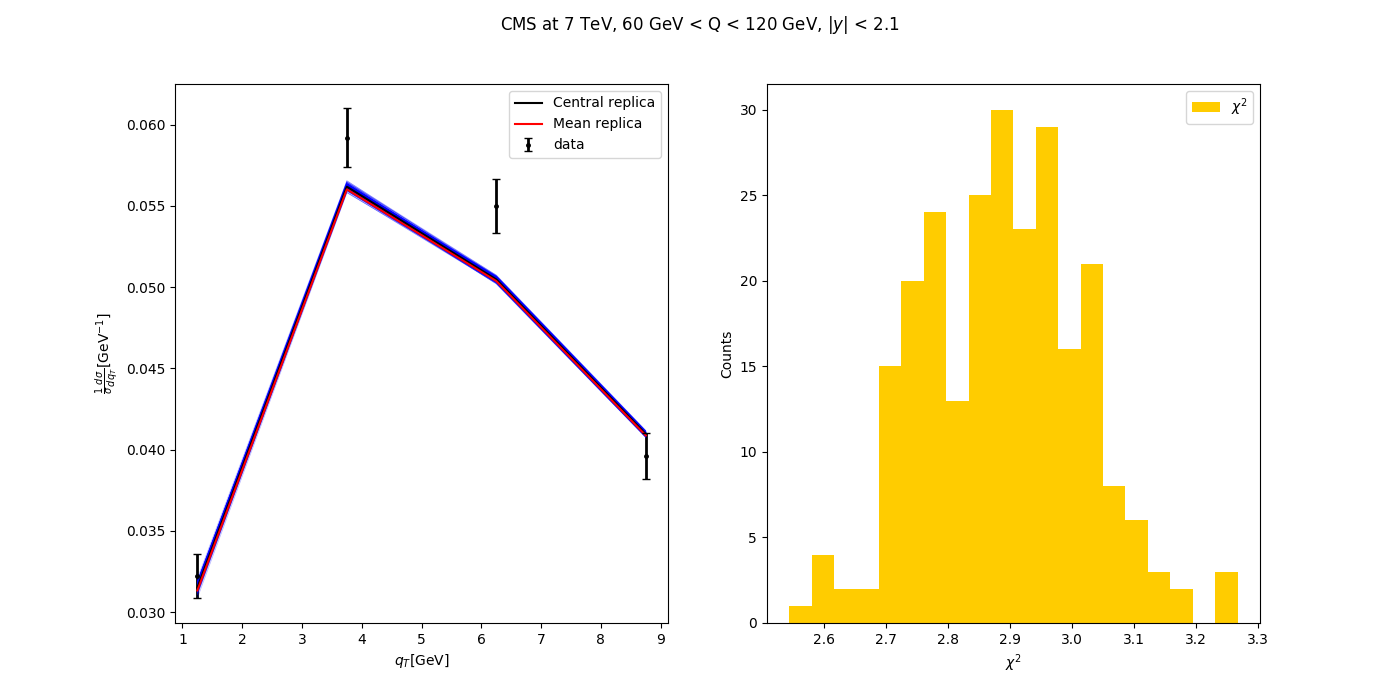
\includegraphics{pngplots/CMS_7TeV.png}
\caption{CMS\_7TeV data-theory comparison}
\end{figure}

\begin{figure}
\centering
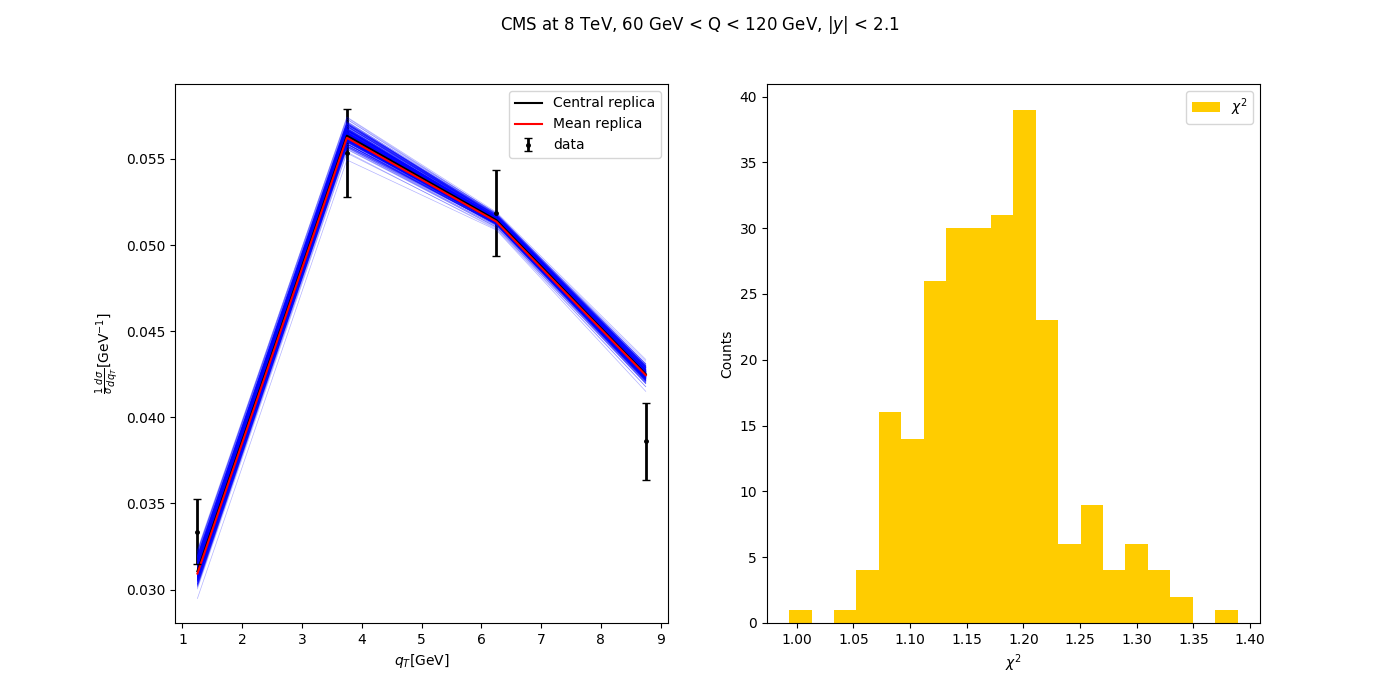
\includegraphics{pngplots/CMS_8TeV.png}
\caption{CMS\_8TeV data-theory comparison}
\end{figure}

\begin{figure}
\centering
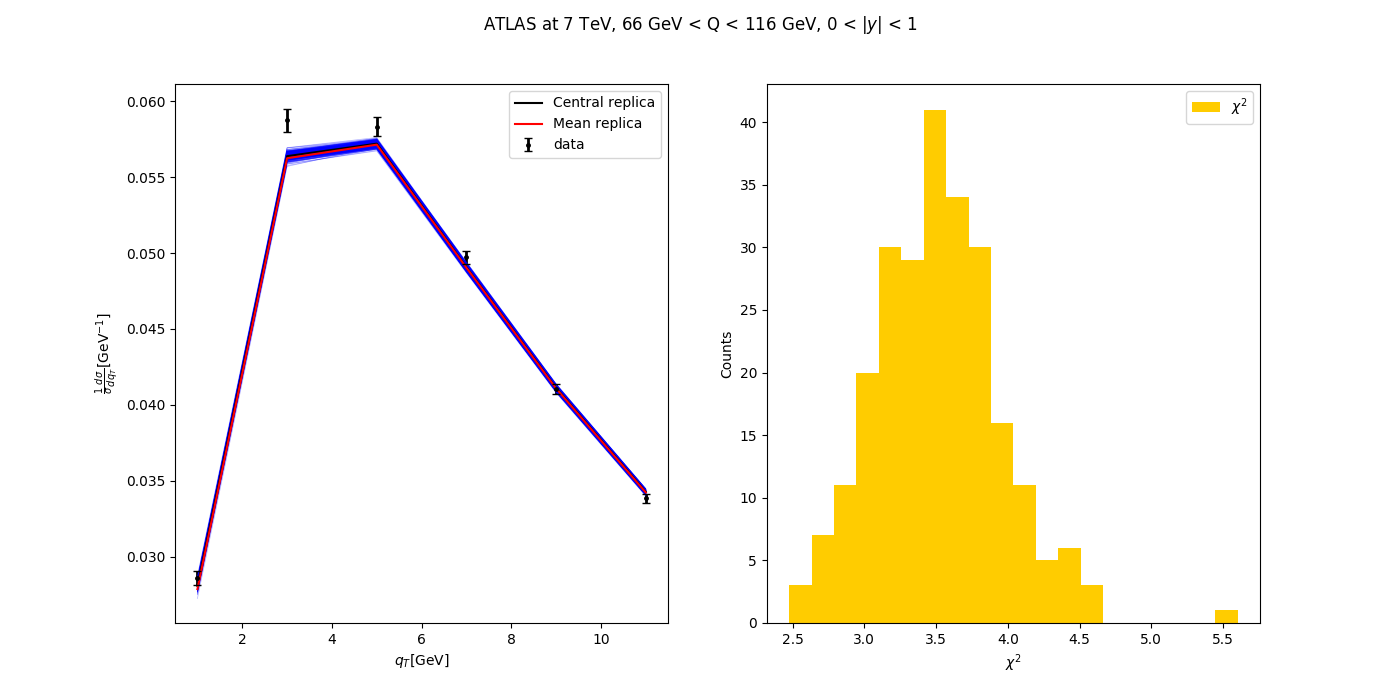
\includegraphics{pngplots/ATLAS_7TeV_y_0_1.png}
\caption{ATLAS\_7TeV\_y\_0\_1 data-theory comparison}
\end{figure}

\begin{figure}
\centering
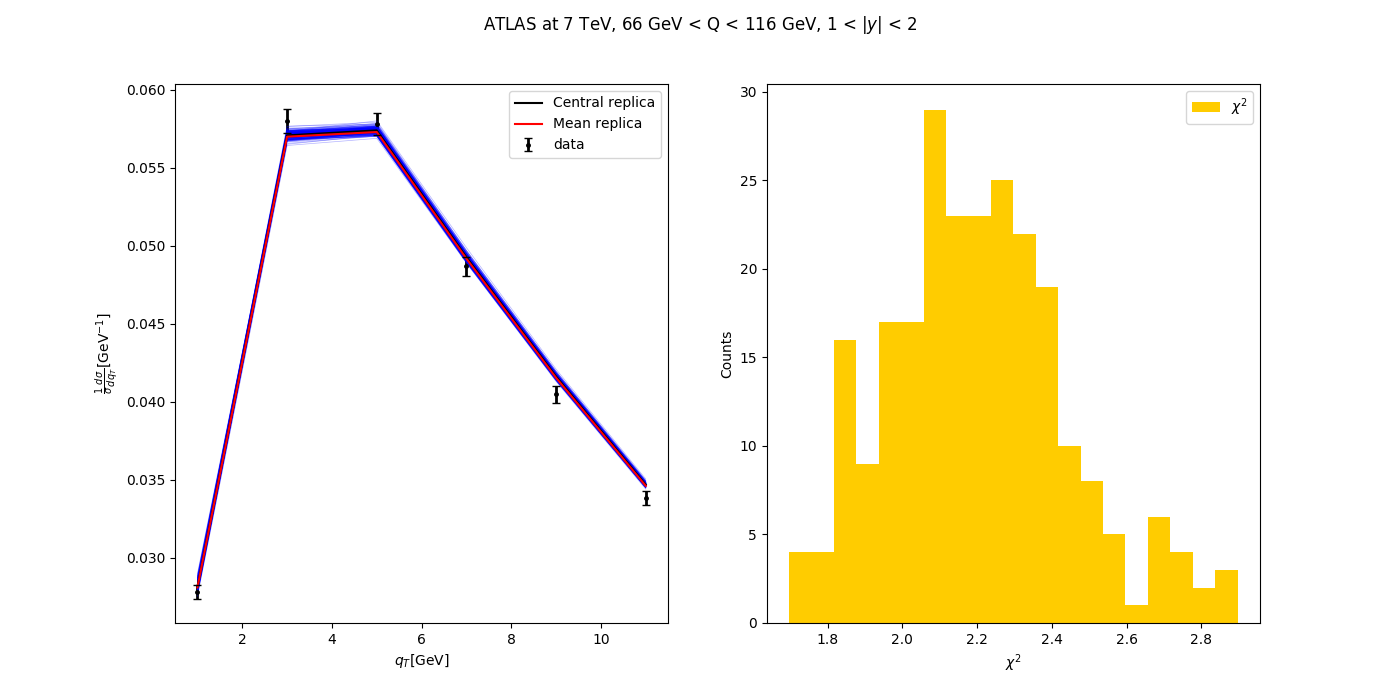
\includegraphics{pngplots/ATLAS_7TeV_y_1_2.png}
\caption{ATLAS\_7TeV\_y\_1\_2 data-theory comparison}
\end{figure}

\begin{figure}
\centering
\includegraphics{pngplots/ATLAS_7TeV_y_2_2.4.png}
\caption{ATLAS\_7TeV\_y\_2\_2.4 data-theory comparison}
\end{figure}

\begin{figure}
\centering
\includegraphics{pngplots/ATLAS_8TeV_y_0_0.4.png}
\caption{ATLAS\_8TeV\_y\_0\_0.4 data-theory comparison}
\end{figure}

\begin{figure}
\centering
\includegraphics{pngplots/ATLAS_8TeV_y_0.4_0.8.png}
\caption{ATLAS\_8TeV\_y\_0.4\_0.8 data-theory comparison}
\end{figure}

\begin{figure}
\centering
\includegraphics{pngplots/ATLAS_8TeV_y_0.8_1.2.png}
\caption{ATLAS\_8TeV\_y\_0.8\_1.2 data-theory comparison}
\end{figure}

\begin{figure}
\centering
\includegraphics{pngplots/ATLAS_8TeV_y_1.2_1.6.png}
\caption{ATLAS\_8TeV\_y\_1.2\_1.6 data-theory comparison}
\end{figure}

\begin{figure}
\centering
\includegraphics{pngplots/ATLAS_8TeV_y_1.6_2.png}
\caption{ATLAS\_8TeV\_y\_1.6\_2 data-theory comparison}
\end{figure}

\begin{figure}
\centering
\includegraphics{pngplots/ATLAS_8TeV_y_2_2.4.png}
\caption{ATLAS\_8TeV\_y\_2\_2.4 data-theory comparison}
\end{figure}

\begin{figure}
\centering
\includegraphics{pngplots/ATLAS_8TeV_Q_46_66.png}
\caption{ATLAS\_8TeV\_Q\_46\_66 data-theory comparison}
\end{figure}

\begin{figure}
\centering
\includegraphics{pngplots/ATLAS_8TeV_Q_116_150.png}
\caption{ATLAS\_8TeV\_Q\_116\_150 data-theory comparison}
\end{figure}

\end{document}
